%!TEX program = xelatex
% 完整编译: xelatex -> biber/bibtex -> xelatex -> xelatex
\documentclass[lang=cn,a4paper,newtx]{elegantpaper}
\title{深度学习环境配置与使用方法教程}
\author{张庚 \\ 上海工程技术大学}
\institute{电子电气工程学院7719实验室}

\version{version 1.1}
\date{\zhdate{2023/12/24}}

% 本文档命令
\usepackage{array}
\usepackage{subcaption}
\usepackage{longtable}
\newcommand{\ccr}[1]{\makecell{{\color{#1}\rule{1cm}{1cm}}}}
% \addbibresource[location=local]{reference.bib} % 参考文献,不要删除

\begin{document}

\maketitle

\tableofcontents
\newpage

\section{前言}
本篇文档介绍的是实验室对已有的硬件设备进行系统、软件安装和使用的教程,根据日常实验室使用过程中出现的问题以及使用习惯,以及本人在实验经验、经历总结出以下的系统使用过程,以方便组内的同学使用。

\subsection{操作系统的选择与安装过程}
Linux 操作系统有很多选择,一般分为以下几个派别的:Debian系(例如Debian、Ubuntu、Deepin、Kali等)、Fedora系(RedHat、Fedora、CentOS等)、Arch系、Gentoo系、SUSE系等。
介于生态、可维护性、开源免费性考虑,我们不选择基于滚动版本的操作系统(例如ArchLinux、CentOS Stream等),商业版本操作系统(RedHat、Oracle Linux等等)、自配置源码编译系统(Gentoo、Funtoo甚至LFS操作系统等等)、包括其他系列的较难使用的操作系统(例如NixOS等),
我们首要考虑的是兼容性、广泛性和实用性,所以在日常实验中,大家可以选择以下系列的操作系统:
\begin{itemize}
  \item 基于Debian的系统:Linux Mint、Ubuntu、Ubuntu衍生版;
  \item 基于Fedora的系统:Fedora、Rocky、Alma;
\end{itemize}


以上的操作系统均具有较好的开源性、稳定性,并且社区教程和资源比较多,所以选择以上的操作系统作为自己的开发系统。
在大模型部署的容器中,有些教程选择较为轻量级的Alpine Linux作为Docker容器内部的操作系统环境,这也是可以的,目的就是尽一切可能简化Docker容器内的操作系统配置文件大小。
Ubuntu 建议选择16.04,18.04,20.04,22.04或者24.04这几个版本。在本服务器上我们选择了Ubuntu衍生版的操作系统,国产Ubuntu Kylin22.04,对Windows应用具有较好的兼容性,Windows味道的桌面,特别是对于小白友好。

Windows 操作系统选择Windows10或者是Windows Server 2019服务器版操作系统。

\subsection{Linux系统安装过程}

Debian系列操作系统首选Ubuntu22.04,也可以选择基于这个系列的衍生版,在官网或者各大镜像站下载,例如清华大学镜像站、中科大镜像站、阿里镜像站等等,
例如清华大学镜像站下载Ubuntu 22.04操作系统,注意选择正确的架构,基于自己笔记本和服务器的操作系统一般都是x86系列的,这里选择64位操作的x86操作系统amd64架构,如图所示:

\begin{figure}[hbpt]
    \centering
    \subfloat[清华大学镜像站]{
      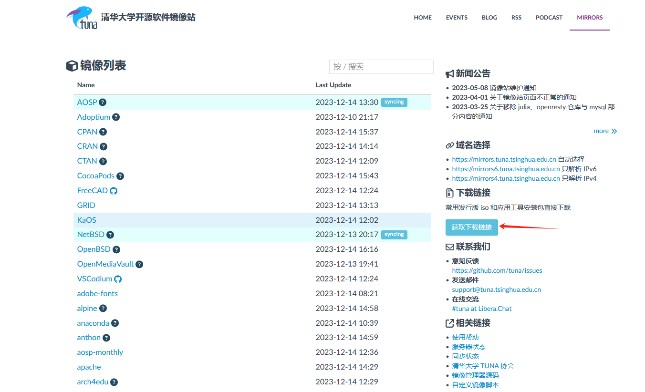
\includegraphics[width=0.48\textwidth]{web1.jpg}
      \label{fig:download_web1}
    }
    \subfloat[Ubuntu 22.04下载页面]{
      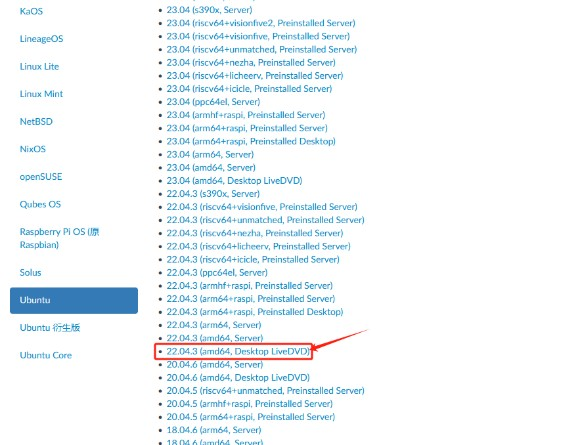
\includegraphics[width=0.48\textwidth]{web2.jpg}
      \label{fig:download_web2}
    }
    \caption{Ubuntu下载页面}
    \label{fig:download_webpage}
\end{figure}


在Windows下使用UltraISO工具或者BalenaEtcher镜像刻录工具(如图所示),将其写入到U盘中,得到系统的启动盘,U盘刻录需要花费大概10-20分钟或者更少的时间。


\begin{figure}[hbpt]
  \centering
  \subfloat[UltraISO工具]{
    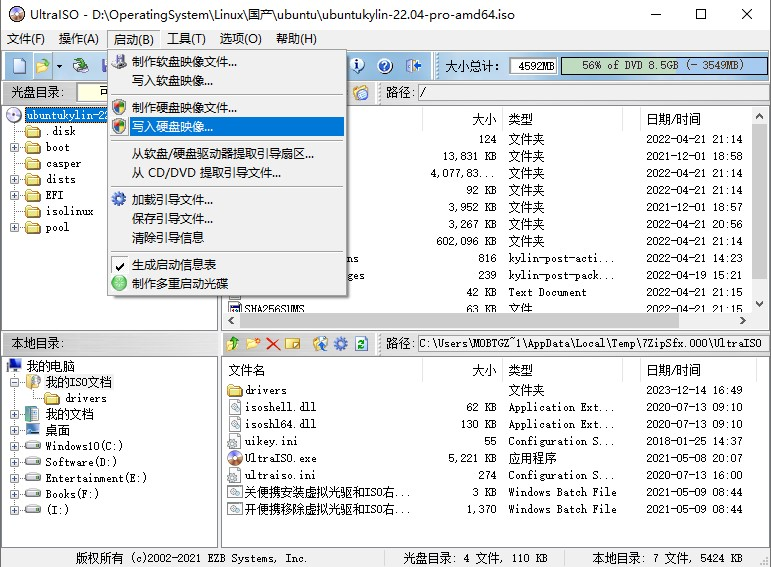
\includegraphics[width=0.48\textwidth]{writeimg1.jpg}
    \label{fig:writeimg1}
  }
  \subfloat[BalenaEtcher工具]{
    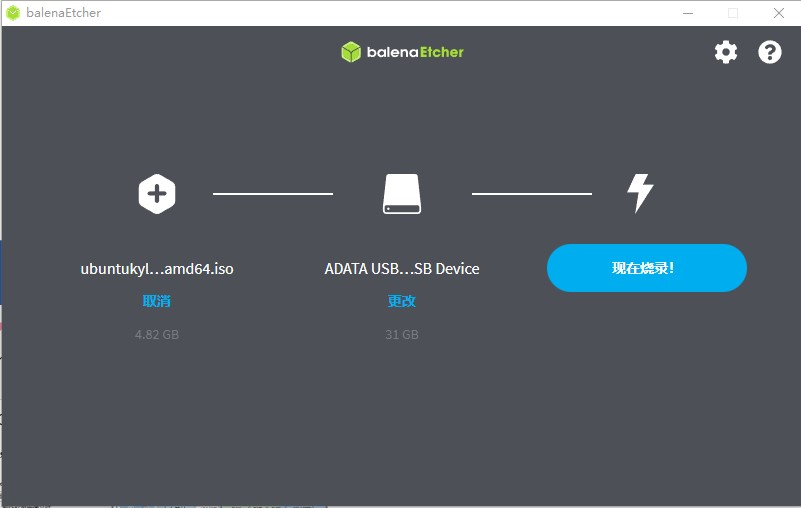
\includegraphics[width=0.48\textwidth]{writeimg2.jpg}
    \label{fig:writeimg2}
  }
  \caption{刻录工具介绍}
  \label{fig:write_imgs_page}
\end{figure}

当然也可以选择功能强大的Ventoy工具,如图\ref{fig:ventoy}所示安装,将Ventoy工具安装在U盘之后,直接将下载好ISO文件丢到Ventoy分区当中即可,具体安装步骤可以参考Ventoy官方网站。

\begin{figure}[hbpt]
  \centering
  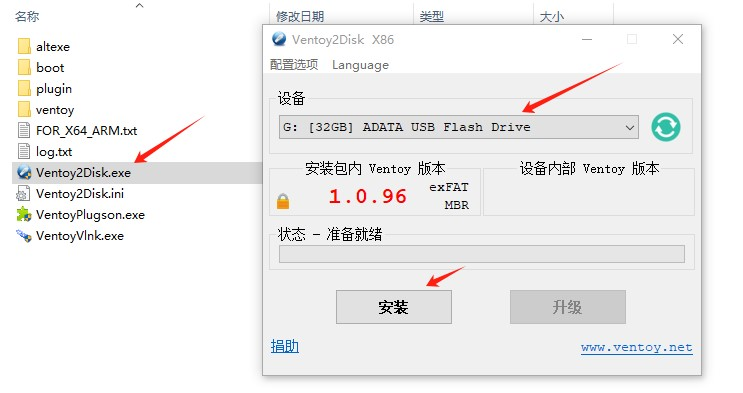
\includegraphics[width=0.8\textwidth]{ventoy.jpg}
  \caption{Ventoy工具安装}
  \label{fig:ventoy}
\end{figure}

刻录完成之后,将U盘插入到电脑上,开机按Del按键(具体按照主板型号)进入BIOS界面,关闭Secure Boot选项,并将启动方式改为UEFI启动方式,第一启动项改为U盘启动,重启工作站即可进入到U盘的系统。
当然有些设备按F12或ESC按键(具体参照主板型号)可以直接进入U盘系统。

进入U盘中的Ubuntu预安装系统,按照步骤即可。
需要注意的是,选择英文作为系统默认的语言,免去日后开发过程中的一些不必要的麻烦;选择最小化安装的方式,这样可以出去一些不必要的软件;安装过程中选择将一些软件包更新skip掉,或者断开网线进行安装操作系统,这些软件包更新实际上在系统安装完成之后联网更新也是可以的;
交换分区按照实际大小来进行设置,也可以不进行设置处理。如若不设置的话,系统会在根据目录下设置一个相当于交换分区的文件用于和内存之间的交换。一般情况下,内存足够大不需要设置交换分区的,交换分区相当于在Windows系统中的虚拟内存大小的设置。

\subsubsection{安装系统之后的操作}
首先备份操作系统原来的源
\begin{lstlisting}[language=bash]
cp /etc/apt/sources.list  /etc/apt/sources.list.bak
\end{lstlisting}

然后将源的内容更换为国内镜像源,这里我们可以选择中科大镜像源、清华镜像源或者是阿里云镜像源,我们这里选择中科大镜像源:

\begin{lstlisting}[language=bash]
sudo nano /etc/apt/sources.list
\end{lstlisting}

更改为以下的内容
\begin{lstlisting}[language=bash]
# 默认注释了源码仓库,如有需要可自行取消注释
deb https://mirrors.ustc.edu.cn/ubuntu/ jammy main restricted universe multiverse
# deb-src https://mirrors.ustc.edu.cn/ubuntu/ jammy main restricted universe multiverse

deb https://mirrors.ustc.edu.cn/ubuntu/ jammy-security main restricted universe multiverse
# deb-src https://mirrors.ustc.edu.cn/ubuntu/ jammy-security main restricted universe multiverse

deb https://mirrors.ustc.edu.cn/ubuntu/ jammy-updates main restricted universe multiverse
# deb-src https://mirrors.ustc.edu.cn/ubuntu/ jammy-updates main restricted universe multiverse

deb https://mirrors.ustc.edu.cn/ubuntu/ jammy-backports main restricted universe multiverse
# deb-src https://mirrors.ustc.edu.cn/ubuntu/ jammy-backports main restricted universe multiverse

# 预发布软件源,不建议启用
# deb https://mirrors.ustc.edu.cn/ubuntu/ jammy-proposed main restricted universe multiverse
# deb-src https://mirrors.ustc.edu.cn/ubuntu/ jammy-proposed main restricted universe multiverse  
\end{lstlisting}

使用国内镜像站的源作为系统源的目的是,在下载源软件能够更快更好,更新系统也较为方便,以防止网络延迟。然后更新源:
\begin{lstlisting}[language=bash]
sudo apt update # 更新源
sudo apt upgrade # 升级软件包  
\end{lstlisting}

\subsubsection{安装python3}
注意这里安装的是系统中python3和pip环境,与后面conda中python环境是不一致的,若不需要系统环境下的python环境可以跳过这个步骤。
\begin{lstlisting}[language=bash]
sudo apt install python3 python3-pip python3-dev python3-virtualenv
\end{lstlisting}

更改pip配置,将安装好的python中pip源的配置更换为以下的设置,显得pip安装速度会更快。
下面是用户文件夹配置pip源
\begin{lstlisting}[language=bash]
  cd ~
  mkdir .pip
  # 编辑文件pip.conf
  sudo nano ~/.pip/pip.conf  
\end{lstlisting}

更换为以下的内容
\begin{lstlisting}[language=bash]
[global]
index-url = https://mirrors.aliyun.com/pypi/simple/
[install]
trusted-host=mirrors.aliyun.com
\end{lstlisting}

下面是root用户配置pip源
\begin{lstlisting}[language=bash]
  sudo mkdir /root/.pip
  # 编辑文件pip.conf
  sudo nano /root/.pip/pip.conf
\end{lstlisting}

创建软链接(非必须)

\begin{lstlisting}[language=bash]
  # 把原来的python软链接删掉
  sudo rm /usr/bin/python
  # 新建一个软链接
  sudo ln -s /usr/bin/python3 /usr/bin/python
  sudo ln -s /usr/bin/pip3 /usr/bin/pip
\end{lstlisting}

当然上述创建软链接也是非必须的,在从系统源上安装python3时候就已经将其软链接建立好了。


\subsection{Windows10 安装过程}
在MSDN上可以下载Windows10或者Windows Server2019原版镜像,同时再下载一个WinPE ISO镜像,并将WinPE用UltraISO或者BalenaEtcher工具将ISO文件刻录到U盘上,然后进入U盘系统之后,使用WinNTSetup工具对操作系统进行安装。
由于在Windows系统安装过程极为简便这里就不再过多进行叙述。


\section{SSH远程登录等配置}
\subsection{SSH远程登录}
一般情况下,Ubuntu 系统中会默认安装好SSH环境,如果没有SSH,则通过以下的方式进行安装
\begin{lstlisting}[language=bash]
sudo apt install openssh-server # 安装openssh服务器端
sudo apt install openssh-client # 安装openssh客户端
\end{lstlisting}

可以用以下的命令启动ssh,或者是开机启动SSH:
\begin{lstlisting}[language=bash]
sudo /etc/init.d/sshd restart #重启SSH服务
sudo /etc/init.d/sshd stop #停止SSH服务
sudo /etc/init.d/sshd start #开启SSH服务
\end{lstlisting}

当然现在大多数Linux 为systemd初始化的操作系统,openRC方式较少,也可以通过以下的方式进行重启服务:

\begin{lstlisting}[language=bash]
sudo systemctl restart ssh#重启SSH服务
sudo systemctl stop ssh #停止SSH服务
sudo systemctl start ssh #开启SSH服务
sudo systemctl enable ssh #开机启动SSH服务
sudo systemctl disable ssh #禁用SSH服务
\end{lstlisting}

可以通过以下的命令查看SSH服务是否启动
\begin{lstlisting}[language=bash]
sudo systemctl status ssh # 查看ssh服务状态
\end{lstlisting}

使用SSH登录用以下的命令即可以登录:
\begin{lstlisting}[language=bash]
ssh -p port_number username@ipaddress
\end{lstlisting}
其中-p表示的是指向的端口号名称,默认为22;username为远程主机的用户名,ipaddress为远程主机的IP地址。连接上之后,就可以当做Linux用户主机使用。


\subsection{STFP文件传输工具(选看)}
在计算机领域,SSH文件传输协议(英语:SSH File Transfer Protocol,也称Secure File Transfer Protocol,中文:安全文件传送协议,英文:Secure FTP或字母缩写:SFTP)是一数据流连线,提供文件存取、传输和管理功能的网络传输协议。与 FTP 协议相比,在几乎所有情况下,SFTP 都比 FTP 更可靠,因为它具有潜在的安全功能并且能够搭载 SSH 连接。 FTP 是一种不安全的协议,只能在有限的情况下或您信任的网络上使用。

一般远程客户端配置好了SSH,就可以使用SFTP协议传输文件。如果使用了自定义的SSH 端口号(默认为22),打开SFTP会话时可以设定端口号
\begin{lstlisting}[language=bash]
sftp -oPort=custom_port username@ ipaddress
\end{lstlisting}

几个常见的使用方法如下

\begin{itemize}
  \item \textbf{获取帮助:}可以通过以下的命令查看SFTP参数使用方法
  \begin{lstlisting}[language=bash]
sftp> help
或
sftp> ?
  \end{lstlisting}
  输出结果如下所示
  \begin{lstlisting}[language=bash]
sftp> help
Available commands:
bye                                Quit sftp
cd path                            Change remote directory to 'path'
chgrp [-h] grp path                Change group of file 'path' to 'grp'
chmod [-h] mode path               Change permissions of file 'path' to 'mode'
chown [-h] own path                Change owner of file 'path' to 'own'
df [-hi] [path]                    Display statistics for current directory or
                                 filesystem containing 'path'
exit                               Quit sftp
get [-afpR] remote [local]         Download file
help                               Display this help text
lcd path                           Change local directory to 'path'
lls [ls-options [path]]            Display local directory listing
lmkdir path                        Create local directory
ln [-s] oldpath newpath            Link remote file (-s for symlink)
lpwd                               Print local working directory
ls [-1afhlnrSt] [path]             Display remote directory listing
lumask umask                       Set local umask to 'umask'
mkdir path                         Create remote directory
progress                           Toggle display of progress meter
put [-afpR] local [remote]         Upload file
pwd                                Display remote working directory
quit                               Quit sftp
reget [-fpR] remote [local]        Resume download file
rename oldpath newpath             Rename remote file
reput [-fpR] local [remote]        Resume upload file
rm path                            Delete remote file
rmdir path                         Remove remote directory
symlink oldpath newpath            Symlink remote file
version                            Show SFTP version
!command                           Execute 'command' in local shell
!                                  Escape to local shell
?                                  Synonym for help
  \end{lstlisting}
  \item \textbf{遍历远程文件系统:}
  我们可以使用一些功能类似于 shell 命令的命令来浏览远程系统的文件层次结构。但是SFTP并不完全是shell的使用方法,从命令上就可以看出并不一样。
  
  首先,通过找出我们当前在远程系统上的哪个目录来定位自己
  \begin{lstlisting}[language=bash]
sftp>pwd
Remote working directory: /home/sesame
  \end{lstlisting}
  查看远程系统当前目录的内容
  \begin{lstlisting}[language=bash]
sftp>ls
Cognata                                                                                    Desktop                                                                                    
Documents                                                                                  Downloads                                                                                                                                                                        
nohup.out                                                                                  opt                                                                                        
pangweisong                                                                                qiancj                                                                                     
set_iptables.sh
  \end{lstlisting}
  SFTP其实也实现了一些更重要的可选标志,例如将 -la 添加到 ls 以查看更多文件元数据和权限:
  \begin{lstlisting}[language=bash]
sftp>ls -la
  outputdrwxr-xr-x    5 remote_money   remote_money       4096 Aug 13 15:11 .
  drwxr-xr-x    3 root     root         4096 Aug 13 15:02 ..
  -rw-------    1 remote_money   remote_money          5 Aug 13 15:04 .bash_history
  -rw-r--r--    1 remote_money   remote_money        220 Aug 13 15:02 .bash_logout
  -rw-r--r--    1 remote_money   remote_money       3486 Aug 13 15:02 .bashrc
  drwx------    2 remote_money   remote_money       4096 Aug 13 15:04 .cache
  -rw-r--r--    1 remote_money   remote_money        675 Aug 13 15:02 .profile
  . . .
  \end{lstlisting}
  进入到其他目录
  \begin{lstlisting}[language=bash]
sftp>cd testDirectory
sftp> cd qiancj
  \end{lstlisting}
  \item \textbf{访问本地的文件系统:}
  通过在命令前面加上一个 l(local) 来将命令指向本地文件系统,例如pwd,cd等等。
  \begin{lstlisting}[language=bash]
sftp>lpwd
Local working directory: /home/qiancj
sftp> lcd /home/qiancj/codes/sanjie
  \end{lstlisting}
  \item \textbf{从远程服务器下载文件到本地服务器:}
  从远程系统上下载文件到本地
  \begin{lstlisting}[language=bash]
sftp> get remoteFile
  OutputFetching /home/remote_money/remoteFile to remoteFile
  /home/remote_money/remoteFile      100%   37KB  36.8KB/s   00:01
  \end{lstlisting}
  
  下载到本地并重命名
  \begin{lstlisting}[language=bash]
sftp> get remoteFile localFile
  \end{lstlisting}

get 命令可以增加可选项,比如要拷贝目录及其下所有文件,可以使用-r选项
  \begin{lstlisting}[language=bash]
sftp> get -r someDirectory
  \end{lstlisting}

使用 -P 或 -p 标志维护适当的权限和访问时间
  \begin{lstlisting}[language=bash]
sftp> get -Pr someDirectory
  \end{lstlisting}

  \item \textbf{传输本地文件到远程服务器:}
使用 put 命令:  
  \begin{lstlisting}[language=bash]
sftp> put localFile
  \end{lstlisting}

  传输到远程服务器并重命名
  \begin{lstlisting}[language=bash]
sftp> put localFile remoteFile
  \end{lstlisting}

  传输目录及其下所有文件
  \begin{lstlisting}[language=bash]
put -r localDirectory
  \end{lstlisting}
\end{itemize}

\subsection{XRDP桌面远程登录(选看)}
xrdp是一个微软远程桌面协议(RDP)的开源实现,允许我们通过Xorg协议的图形界面远程控制操作系统。这里使用RDP而不是VNC作为远程桌面,这是因为Windows自带的远程桌面连接软件就可以连接很方便,同时也可以直接实现在主机和远程主机之间的复制粘贴等等操作,比较方便。

安装步骤如下所示:
\begin{lstlisting}[language=bash]
sudo apt install xrdp # 安装xrdp
\end{lstlisting}

安装完成之后xrdp就会自动启动,可以使用以下的命令查看它的状态信息
\begin{lstlisting}[language=bash]
sudo systemctl status xrdp
\end{lstlisting}

设置为开机启动
\begin{lstlisting}[language=bash]
sudo systemctl enable xrdp
\end{lstlisting}

默认情况下,xrdp 使用/etc/ssl/private/ssl-cert-snakeoil.key,它仅仅对ssl-cert用户组成语可读,所以需要运行下面的命令,将xrdp用户添加到这个用户组:
\begin{lstlisting}[language=bash]
sudo adduser xrdp ssl-cert  
sudo systemctl restart xrdp
\end{lstlisting}

\subsection{Samba文件共享(选看)}
我们这里选择的的是SAMBA文件共享服务进行安装,可以通过建立局域网SAMBA服务来实现:
安装SAMBA服务:
\begin{lstlisting}[language=bash]
sudo apt-get install samba samba-common-bin
\end{lstlisting}

配置/etc/samba/smb.conf文件
\begin{lstlisting}[language=bash]
suod nano /etc/samba/smb.conf
\end{lstlisting}

在文件的最后添加以下的内容
\begin{lstlisting}[language=bash]
# 共享文件夹显示的名称
[home]
# 说明信息
comment = WorkStation Storage
# 可以访问的用户
valid users = mobtgzhang,root
# 共享文件的路径
path = /home/mobtgzhang/
# 可被其他人看到资源名称(非内容)
browseable = yes
# 可写
writable = yes
# 新建文件的权限为 664
create mask = 0664
# 新建目录的权限为 775
directory mask = 0775
\end{lstlisting}

可以把配置文件中你不需要的分享名称删除,例如 [homes], [printers] 等。运行这个命令测试一下配置文件是否有错误,根据提示做相应修改:testparm

添加登陆账户并创建密码,必须是 linux 已存在的用户:
\begin{lstlisting}[language=bash]
sudo smbpasswd -a mobtgzhang
\end{lstlisting}

重启samba服务
\begin{lstlisting}[language=bash]
sudo systemctl restart smbd
\end{lstlisting}

\section{深度学习环境配置}

深度学习环境的配置首要的问题是深度学习显卡加速驱动的安装,对于NVIDIA显卡驱动来说是CUDA深度学习加速库,对于AMD显卡来说是ROCm深度学习加速库,其他的计算卡通过对应的教程可以进行安装。
然后在这些驱动和加速库的基础之上可以进一步进行深度学习环境的配置和安装,这里列举了几种显卡/计算卡的配置方法以供参考。

\subsection{NVIDIA 显卡深度学习环境配置}
最为常见的深度学习显卡为NVIDIA显卡,这里一共有两种方法安装NVIDIA驱动,下面分为两个章节介绍这两种方法。

\subsubsection{从源上安装显卡驱动}
首先我们列举出可用显卡信息

\begin{lstlisting}[language=bash]
sudo apt-get update #更新一下源
ubuntu-drivers devices
\end{lstlisting}

它会列举出显卡驱动的信息,选择你想要安装的显卡驱动信息:
\begin{figure}[hbpt]
  \centering
  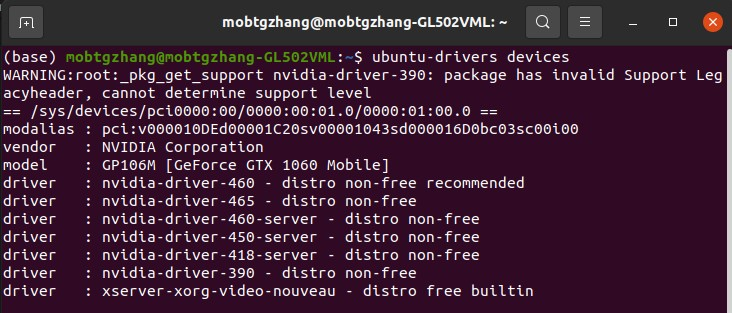
\includegraphics[width=0.8\textwidth]{nv-ubuntu.jpg}
  \caption{Ubuntu 系统下显示的设备信息}
  \label{fig:nv-ubuntu}
\end{figure}

例如安装以下显卡驱动信息:
\begin{lstlisting}[language=bash]
sudo apt-get install nvidia-driver-470
\end{lstlisting}

或者安装对于ubuntu系统的显卡驱动,自动安装驱动程序:
\begin{lstlisting}[language=bash]
sudo ubuntu-drivers autoinstall
\end{lstlisting}

重启电脑,即可以安装成功。

\subsubsection{官网驱动安装}
\begin{enumerate}[label=(\arabic*)]
  \item \textbf{禁用nouveau驱动:} 
  
  nouveau,是一个自由及开放源代码显卡驱动程序,是为Nvidia的显示卡所编写,也可用于属于系统芯片的NVIDIA Tegra系列,此驱动程序是由一群独立的软件工程师所编写。
  但是nouveau开源驱动基本上是不能正常使用的,性能极低。

  首先编辑文件 blacklist.conf:
  \begin{lstlisting}[language=bash]
sudo nano /etc/modprobe.d/blacklist.conf
  \end{lstlisting}

  移动光标,在最后一行添加以下代码:
  \begin{lstlisting}[language=bash]
blacklist nouveau
options nouveau modeset=0
  \end{lstlisting}
  然后ctrl + O保存文件。
  \item \textbf{更新内核文件:}

  注意备份文件,还需要注意自己系统的内核文件,不同版本的Linux内核更新不一样

  \begin{lstlisting}[language=bash]
# 备份内核文件
sudo cp /boot/initrd.img-$(uname -r)$ /boot/initrd.img-$(uname -r)$.bak
# 更新内核文件
sudo update-initramfs -u
# 更新GRUB
sudo update-grub2 # 或者是sudo grub2-mkconfig -o /boot/grub/grub.cfg
# 重启电脑
sudo shutdown -r now
  \end{lstlisting}
  \item \textbf{进入BIOS设置,关闭Secure Boot设置:}
  进入 Secure Boot Menu,将Secure Boot Control 设置为disabled。由于Secure boot带来的一些内核签名验证问题,比较麻烦,所以为简易起见关闭了Secure boot设置。
  \begin{figure}[hbpt]
    \centering
    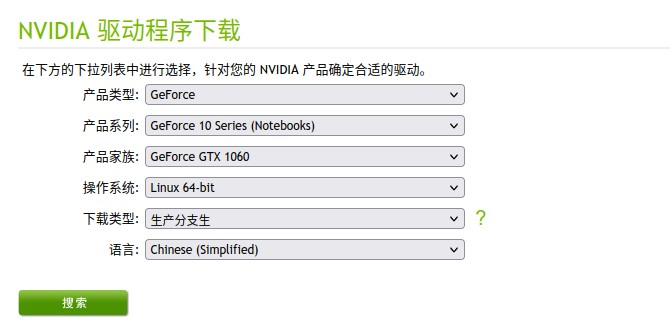
\includegraphics[width=0.8\textwidth]{nv-offical.jpg}
    \caption{NVIDIA 官方网址}
    \label{fig:nv-offical}
  \end{figure}

  从官网下载驱动程序。以我自己的笔记本为例,选择对应的版本即可。

  然后进行安装
  \begin{lstlisting}[language=bash]
    sudo bash NVIDIA-Linux-x86_64-{你的NVIDIA驱动版本号}.run --no-x-check --no-nouveau-check --no-opengl-files
  \end{lstlisting}

  参数的含义如下:
  \begin{itemize}
    \item \textbf{--no-x-check}:不检查X服务是否运行;
    \item \textbf{--no-nouveau-check}:不检查nouveau驱动是否运行;
    \item \textbf{--no-opengl-files}:只安装驱动文件,不安装OpenGL文件  
  \end{itemize}

  这样再reboot,就不会出现循环登录的问题。

\end{enumerate}

\subsubsection{检查驱动是否安装成功}
检查NVIDIA显卡驱动程序是否安装成功,可启动nvidia-smi 进行查看(如图\ref{fig:nvidia-smi-ukylin}所示):

\begin{figure}[hbpt]
  \centering
  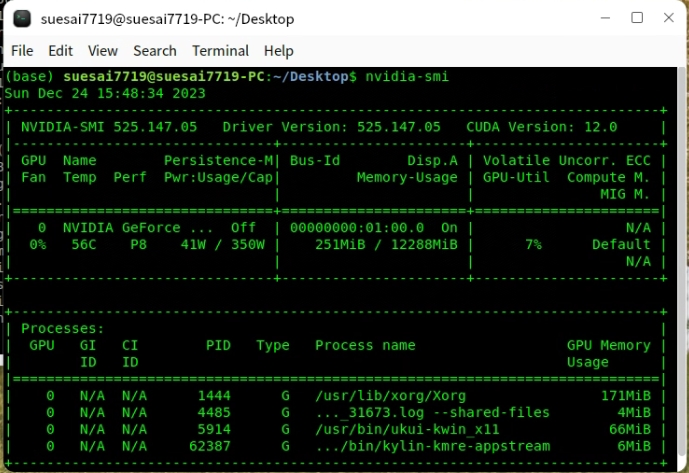
\includegraphics[width=0.8\textwidth]{ukylin-nvidia-smi.jpg}
  \caption{nvidia-smi 查看显卡驱动信息}
  \label{fig:nvidia-smi-ukylin}
\end{figure}

也可以启动nvidia-settings 进行查看(如图\ref{fig:ubuntu-nvidia-settings}所示):

\begin{figure}[hbpt]
  \centering
  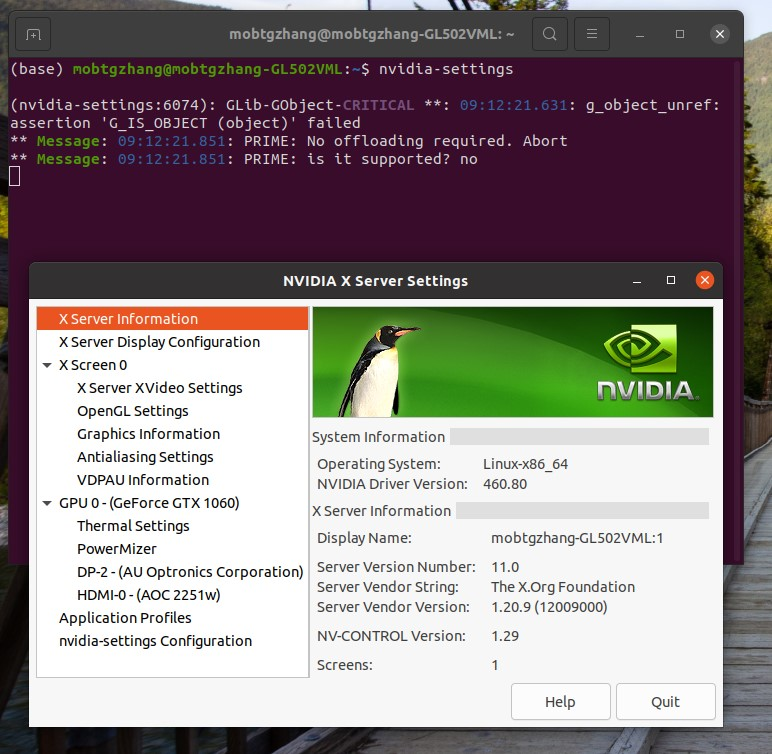
\includegraphics[width=0.6\textwidth]{ubuntu-nvidia-settings.jpg}
  \caption{nvidia-settings 设置查看显卡驱动信息}
  \label{fig:ubuntu-nvidia-settings}
\end{figure}

\subsubsection{CUDA 安装}
因为编译cuda程序需要GCC版本低一点的编译器,否则会有以下的一些错误:
\begin{lstlisting}[language=bash]
Error: unsupported compiler: 8.2.0. Use --override to override this check.
\end{lstlisting}

对于Ubuntu22.04来说,源上最低版本的GCC工具为GCC-7.5.0,所以我们这里使用GCC7版本的编译器,安装对应的GCC编译器。
\begin{lstlisting}[language=bash]
sudo apt install gcc-7 g++-7
\end{lstlisting}

查看是否安装成功
\begin{lstlisting}[language=bash]
cd /usr/bin
ls -l gcc* # 显示gcc编译器
ls -l g++* # 显示g++编译器
gcc -v # 查看gcc是否安装成功
g++ -v # 查看g++是否安装成功
\end{lstlisting}

如果查看gcc,g++命令当前的版本并非gcc-7和g++-7,那么就需要创建软链接
\begin{lstlisting}[language=bash]
sudo mv /usr/bin/gcc /usr/bin/gcc.bak
sudo ln -s /usr/bin/gcc-7 /usr/bin/gcc
sudo mv /usr/bin/g++ /usr/bin/g++.bak
sudo ln -s /usr/bin/g++-7 /usr/bin/g++
\end{lstlisting}

对于Ubuntu22.04来说,源上最低版本的GCC工具为GCC-7.5.0,所以我们这里使用GCC7版本的编译器,安装对应的GCC编译器。

下载CUDA run文件见官网,为兼容方便我们这里安装了cuda-11.2。
\begin{lstlisting}[language=bash]
wget https://developer.download.nvidia.com/compute/cuda/11.2.0/local_installers/cuda_11.2.0_460.27.04_linux.run
sudo sh cuda_11.2.0_460.27.04_linux.run
\end{lstlisting}

注意!!!!安装时候会提示安装它提示安装的显卡驱动,一定要选择no,否则会出现显卡驱动冲突,无法进入桌面环境。

若在安装过程中缺少一些库文件,例如libGL.so等等文件,可能会出现如下错误:
\begin{lstlisting}[language=bash]
Missing recommended library: libGLU.so
Missing recommended library: libX11.so
Missing recommended library: libXi.so
Missing recommended library: libXmu.so
\end{lstlisting}

可以通过以下的命令安装对应的库文件:
\begin{lstlisting}[language=bash]
sudo apt-get install libglu1-mesa libxi-dev libxmu-dev libglu1-mesa-dev
\end{lstlisting}
配置CUDA对应的环境变量,编辑文件bashrc
\begin{lstlisting}[language=bash]
sudo nano ~/.bashrc
\end{lstlisting}

\note{~/.bashrc文件普通用户变量环境文件,如果是root用户,需要修改为/root/.bashrc文件。另外,不要改/etc/profile 文件,这里是整个系统环境变量文件,如果非得需要添加系统环境变量,可以直接在文件夹/etc/profile.d/下添加对应的.sh文件,这样就可以添加系统环境变量了。}

并添加以下内容
\begin{lstlisting}[language=bash]
export PATH=/usr/local/cuda-11.2/bin${PATH:+:$PATH}
export LD_LIBRARY_PATH=/usr/local/cuda-11.2/lib64${LD_LIBRARY_PATH:+:${LD_LIBRARY_PATH}}
\end{lstlisting}

\note{这里的CUDA安装路径为/usr/local/cuda-11.2,如果安装的是其他版本的CUDA,需要修改为对应的版本号。}

使得文件生效
\begin{lstlisting}[language=bash]
source ~/.bashrc
\end{lstlisting}

查看cuda 是否安装成功以及是否添加到环境变量当中
\begin{lstlisting}[language=bash]
nvcc -V
\end{lstlisting}

显示以下的信息

\begin{figure}[hbpt]
  \centering
  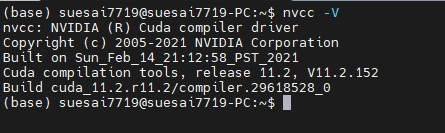
\includegraphics[width=0.8\textwidth]{nvcc.jpg}
  \caption{NVCC 命令显示的内容}
  \label{fig:ubuntu-nvcc}
\end{figure}

另外一种方法是直接在源上安装cuda即可,对于Ubuntu22.04来说,源上的CUDA版本为11.5版本。
\begin{lstlisting}[language=bash]
sudo apt install nvidia-cuda-toolkit
\end{lstlisting}

\subsubsection{CUDNN安装}
官网下载cudnn文件,并解压,注意对应版本的cuda的cudnn,这里是cuda11.2对应的文件
\begin{lstlisting}[language=bash]
tar -xzvf cudnn-11.2-linux-x64-v8.4.15.tgz
sudo cp cuda/include/cudnn* /usr/local/cuda/include
sudo cp cuda/lib64/libcudnn* /usr/local/cuda/lib64
sudo chmod a+r /usr/local/cuda/include/cudnn.h /usr/local/cuda/lib64/libcudnn*
\end{lstlisting}

查看cuda是否安装成功以及是否添加到环境变量当中,cudnn是否安装成功
\begin{lstlisting}[language=bash]
cat  /usr/local/cuda/version.json
cat /usr/local/cuda/include/cudnn_version.h | grep CUDNN_MAJOR -A 2
\end{lstlisting}

至此,CUDNN即可安装到系统当中。当然也可以从源上安装CUDNN,Ubuntu22.04源上的版本为8.2.4.15。
\begin{lstlisting}[language=bash]
sudo apt install nvidia-cudnn
\end{lstlisting}

\subsection{AMD显卡深度学习环境配置(选看)}
AMD显卡也是可以进行深度学习环境搭建的,对于RX5700, RX6600, RX6750xt, RX7900XTX等这些系列的显卡均可以进行深度学习环境搭建。这里以最新版本ROCM5.7.1为例子。
首先,下载并转换包签名密钥
\begin{lstlisting}[language=bash]
sudo mkdir --parents --mode=0755 /etc/apt/keyrings
wget https://repo.radeon.com/rocm/rocm.gpg.key -O - | \
    gpg --dearmor | sudo tee /etc/apt/keyrings/rocm.gpg > /dev/null
\end{lstlisting}

对于Ubuntu22.04,在apt额外源库中添加ROCm源:
\begin{lstlisting}[language=bash]
# jammy版本的Kernel驱动仓库源
sudo tee /etc/apt/sources.list.d/amdgpu.list <<'EOF'
deb [arch=amd64 signed-by=/etc/apt/keyrings/rocm.gpg] https://repo.radeon.com/amdgpu/5.7.1/ubuntu jammy main
EOF
# jammy版本的ROCm驱动仓库源
sudo tee /etc/apt/sources.list.d/rocm.list <<'EOF'
deb [arch=amd64 signed-by=/etc/apt/keyrings/rocm.gpg] https://repo.radeon.com/rocm/apt/debian jammy main
EOF
# 与系统包相比,更好是来自rocm存储库的包
echo -e 'Package: *\nPin: release o=repo.radeon.com\nPin-Priority: 600' | sudo tee /etc/apt/preferences.d/rocm-pin-600
\end{lstlisting} 

然后更新源
\begin{lstlisting}[language=bash]
sudo apt update
\end{lstlisting}

安装rocm-hip-libraries元包。这包含大多数常见ROCm应用程序的依赖项,然后重启操作系统。
\begin{lstlisting}[language=bash]
sudo apt install rocm-hip-libraries
sudo reboot
\end{lstlisting}

这样ROCm机器学习加速库安装完成。可以通过rocm-smi命令查看安装和ROCm运行的情况:
\begin{figure}[hbpt]
  \centering
  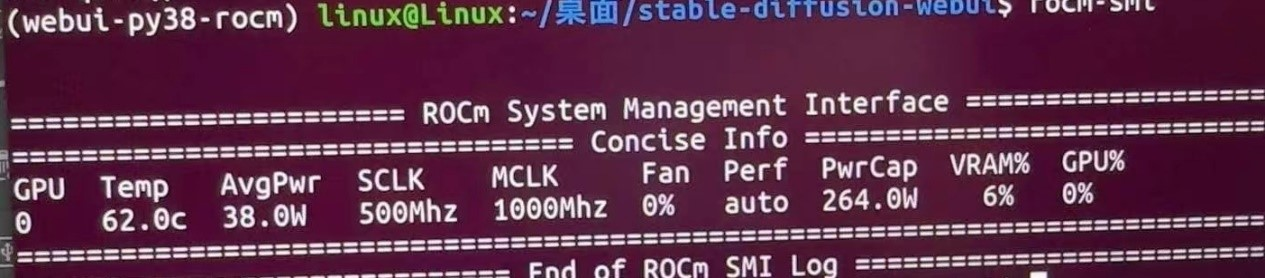
\includegraphics[width=0.8\textwidth]{rocm.jpg}
  \caption{rocm-smi 命令显示的内容}
  \label{fig:ubuntu-rocm-smi}
\end{figure}

详细的安装教程可以参考其官网\footnote{\url{https://rocmdocs.amd.com/en/latest/Installation_Guide/Installation-Guide.html}}。

\subsection{华为昇腾Altas300系列AI加速卡深度学习环境配置(选看)}
(待补充)
\subsection{寒武纪S370系列AI加速卡深度学习环境配置(选看)}
(待补充)
\subsection{燧原T20、T21加速卡深度学习环境配置(选看)}
(待补充)
\subsection{摩尔线程S70、S80AI加速卡深度学习环境配置(选看)}
(待补充)
\section{深度学习框架环境安装}
深度学习是一个非常大的领域,有很多的深度学习框架,不同的语言中也有不同的安装方式,包括Python、Julia、lua等等。这里我们主要介绍Python、Julia、rust、go等几种语言的深度学习框架的安装方法。
\subsection{Python深度学习环境配置}
深度学习框架有很多种,这里我们主要介绍几种常见的深度学习框架的安装方法,包括Pytorch、Tensorflow、Jax、Mindspore、MXNet、Theano等等。这里我们主要介绍Pytorch和Tensorflow的安装方法,其他的框架的安装详细方法可以参考官网的安装教程。
\subsubsection{Miniconda3 安装配置}
Miniconda是一个Anaconda的轻量级替代,默认只包含了python和conda,但是可以通过conda命令来安装所需要的包。Miniconda的安装非常简单,只需要下载对应的安装包,然后运行安装即可。
下载地址可以选择国内的镜像站地址,文件目录位置在anaconda/miniconda3/ 这个文件目录下,例如在清华镜像站地址。
\begin{figure}[hbpt]
  \centering
  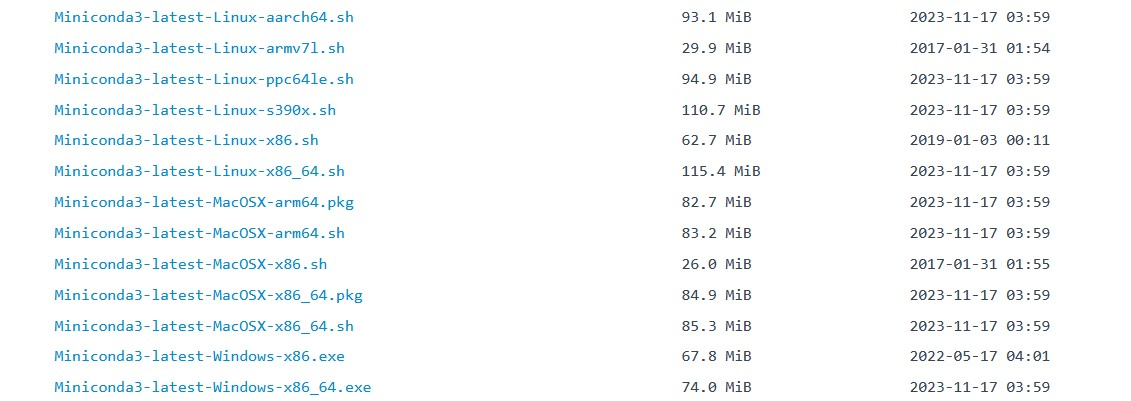
\includegraphics[width=0.8\textwidth]{miniconda-tunhua.jpg}
  \caption{清华镜像站Miniconda下载}
  \label{fig:miniconda-tunhua}
\end{figure}

下载完成之后,直接使用bash安装即可
\begin{lstlisting}[language=bash]
chmod +x Miniconda3-latest-Linux-x86_64.sh
bash Miniconda3-latest-Linux-x86_64.sh
\end{lstlisting}
注意将对应的miniconda安装到的文件目录即可。
最后一个安装步骤是初始化conda,这里选择yes,然后重启终端,即可完成miniconda的安装。
\subsubsection{Python虚拟环境的设置}
这里分为系统虚拟环境使用方法和conda虚拟环境使用方法。
\begin{itemize}
  \item \textbf{系统虚拟环境使用方法:}

当然可以在系统环境中安装对应的虚拟环境包,用以下的命令安装虚拟环境
\begin{lstlisting}[language=bash]
pip3 install virtualenv
\end{lstlisting}

  可以通过以下的命令创建一个虚拟环境
\begin{lstlisting}[language=bash]
python3 -m venv -p /usr/bin/python3
# 或者以下命令
virtualenv -p /bin/python3 venv
\end{lstlisting}

这样就会建立一个名字为venv的虚拟环境。然后激活虚拟环境
\begin{lstlisting}[language=bash]
source path/to/virtualenv/bin/activate
\end{lstlisting}

停止虚拟环境、退出虚拟环境
\begin{lstlisting}[language=bash]
deactivate
\end{lstlisting}
为了更加有效方便管理和安装虚拟环境,所以这里我们可以使用管理工具对虚拟环境进行管理和操作。

安装虚拟环境管理工具
\begin{lstlisting}[language=bash]
pip3 install virtualenvwrapper
\end{lstlisting}

通常virtualenvwrapper有以下的命令进行操作和使用
\begin{lstlisting}[language=bash]
mkvirtualenv venv # 新建虚拟环境
rmvirtualenv venv # 删除虚拟环境
workon # 查看安装的所有虚拟环境
workon venv # 进入或切换虚拟环境
cdsitepackages # 进入虚拟环境的site-packages目录
lssitepackages # 列出site-packages目录的所有软件包
\end{lstlisting}
\item \textbf{conda虚拟环境使用方法:}

conda 虚拟环境的使用方法和系统虚拟环境的使用方法类似,conda默认为base虚拟环境,可以通过以下的命令查看当前的虚拟环境
\begin{lstlisting}[language=bash]
conda info --envs
\end{lstlisting}

可以通过以下的命令创建一个虚拟环境
\begin{lstlisting}[language=bash]
conda create -n venv python=3.8
\end{lstlisting}

这样就会建立一个名字为venv的虚拟环境。其中-n指的是虚拟环境指定虚拟环境名称,python可以指定其中的版本号。
然后激活虚拟环境
\begin{lstlisting}[language=bash]
conda activate venv
\end{lstlisting}

停止虚拟环境、退出虚拟环境
\begin{lstlisting}[language=bash]
conda deactivate
\end{lstlisting}

由于conda默认为官方的镜像源站,所以这里可以将其中的镜像源站修改为国内的镜像源站,例如清华镜像站,这样可以加快下载的速度。
\begin{lstlisting}[language=bash]
conda config --add channels https://mirrors.tuna.tsinghua.edu.cn/anaconda/pkgs/free/
conda config --add channels https://mirrors.tuna.tsinghua.edu.cn/anaconda/pkgs/main/
conda config --add channels https://mirrors.tuna.tsinghua.edu.cn/anaconda/cloud/conda-forge
conda config --add channels https://mirrors.tuna.tsinghua.edu.cn/anaconda/cloud/msys2/
conda config --set show_channel_urls yes
\end{lstlisting}

或者是在~/.condarc文件中添加以下的内容
\begin{lstlisting}[language=bash]
channels:
  - https://mirrors.tuna.tsinghua.edu.cn/anaconda/pkgs/free/
  - https://mirrors.tuna.tsinghua.edu.cn/anaconda/pkgs/main/
  - conda config --add channels https://mirrors.tuna.tsinghua.edu.cn/anaconda/cloud/conda-forge
  - conda config --add channels https://mirrors.tuna.tsinghua.edu.cn/anaconda/cloud/msys2/
show_channel_urls: true
\end{lstlisting}

这样就可以将镜像源站修改为清华镜像站了。

更新conda使用以下的命令
\begin{lstlisting}[language=bash]
conda update conda
\end{lstlisting}
更新conda中base环境中的所有包
\begin{lstlisting}[language=bash]
conda update --all
\end{lstlisting}

\end{itemize}
\subsubsection{Pytorch环境安装}
目前Pytorch分为1.x和2.x两个版本,相较于1.x版本,2.x版本的Pytorch更加的轻量级,2.x版本进一步增强了Python的效率。
pytorch深度学习环境配置一般通过以下的方式进行安装和配置,为了兼容所有深度学习环境,我们这里使用的是cuda11.2版本的配置,
首先创建一个pytorch的虚拟环境,按照以下的方式进行安装:
\begin{lstlisting}[language=bash]
conda create -n pytorch python=3.8
conda activate pytorch
\end{lstlisting}

然后安装pytorch,这里我们选择的是pytorch2.0版本,安装命令如下所示:
\begin{lstlisting}[language=bash]
conda install pytorch torchvision torchaudio cudatoolkit=11.2 -c pytorch -c nvidia
\end{lstlisting}

也可以通过pip安装pytorch,安装命令如下所示:

\begin{lstlisting}[language=bash]
  pip install torch==2.1.0 torchvision==0.16.0 torchaudio==2.1.0 --index-url https://download.pytorch.org/whl/cu118
\end{lstlisting}

安装完成之后,可以通过以下的命令查看pytorch的版本信息
\begin{lstlisting}[language=bash]
python -c "import torch; print(torch.__version__)"
\end{lstlisting}

如果加速卡使用的是AMD显卡,对于基于ROCm5.6 的深度环境,使用以下的命令进行安装:
\begin{lstlisting}[language=bash]
  pip3 install torch torchvision torchaudio --index-url https://download.pytorch.org/whl/rocm5.6
\end{lstlisting}

在项目的处理过程中,我们也使用到了以下的一些基于pytorch的深度学习环境,如下所示
\begin{itemize}
  \item torchvision:计算机图像处理包\footnote{\url{https://pytorch.org/vision/stable/index.html}};
  \item torchaudio:音频处理包\footnote{\url{https://pytorch.org/audio/stable/index.html}};
  \item pytorch\_geometric:图神经网络库(基于networkx图库)\footnote{\url{https://pytorch-geometric.readthedocs.io/en/latest/}};
  
  这个安装过程稍有点复杂,需要安装以下的依赖包:
  \begin{lstlisting}[language=bash]
    pip install --verbose --no-cache-dir torch-scatter
    pip install --verbose --no-cache-dir torch-sparse
    pip install --verbose --no-cache-dir torch-cluster
    pip install --verbose --no-cache-dir torch-spline-conv #(optional)
    pip install torch-geometric
  \end{lstlisting}
  \item DGL:图神经网络库(基于networkx图库)\footnote{\url{https://docs.dgl.ai/index.html}};
  \item allennlp:神经网络库\footnote{\url{https://docs.allennlp.org/main/}};
  \item Transformers:自然语言处理中的预训练模型\footnote{\url{https://huggingface.co/docs/transformers/index}};
  \item 哈工大ltp自然语言处理包\footnote{\url{http://ltp.ai/docs/index.html}};
  \item tensorboardX:神经网络可视化;
  \item skorch:sklearn的pytorch封装;
  \item gpytorch:高斯过程推理库;
  \item botorch:贝叶斯概率推断库;
  \item Pyro:概率推断库;
\end{itemize}

安装过程中注意对应CUDA的版本号安装对应的包文件,这里我们使用的是CUDA11.2版本的深度学习环境,所以安装的包文件也是对应的CUDA11.2版本的包文件。
对于不同的Pytorch库,可以参考对应的Pytorch生态系统\footnote{\url{https://pytorch.org/ecosystem/}}。

测试pytorch CUDA环境是否可以使用:可以使用以下的简单代码测试pytorch的深度学习加速环境是否可以使用
\begin{lstlisting}[language=python]
import torch
print(torch.cuda.is_available())
\end{lstlisting}
若显示True那么就可以使用cuda深度学习加速库。

\subsubsection{Tensorflow环境安装}
首先要注意对应的TensorFlow的GPU版本,如下图\ref{fig:tf-gpu}所示。
\begin{figure}[hbpt]
  \centering
  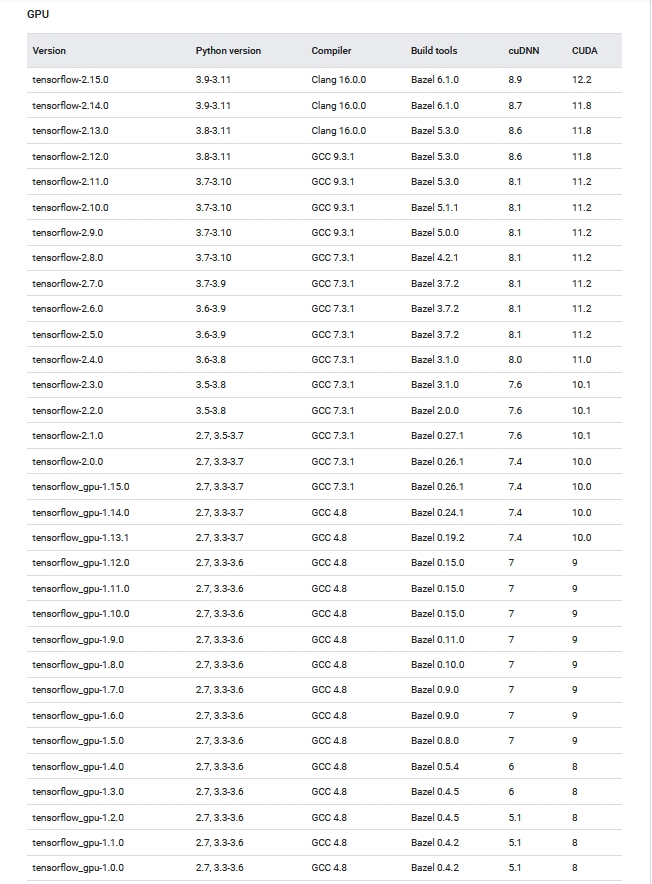
\includegraphics[width=0.8\textwidth]{tf-gpus.jpg}
  \caption{TensorFlow GPU版本对应的CUDA、cuDNN、Python版本}
  \label{fig:tf-gpu}
\end{figure}

这里我们选择的是TensorFlow2.6版本,对应的CUDA版本为11.2,cuDNN版本为8.1,Python版本为3.8。
只需要以下的命令进行安装
\begin{lstlisting}[language=bash]
pip install tensorflow-gpu==2.6.0 # 安装TensorFlow GPU版本
pip install tensorboard  #  神经网络可视化图
\end{lstlisting}

测试GPU是否能使用的方法:
\begin{lstlisting}[language=python]
import tensorflow as tf
device = tf.config.list_physical_devices('GPU')
print(device)
\end{lstlisting}

如果出现了GPU 的列表,就说明GPU深度学习环境已经配置完成。

\newpage

\subsubsection{Jax环境安装}
Jax深度学习框架\footnote{\url{https://jax.readthedocs.io/en/latest/}}是Google开发的一个深度学习框架,它的特点是可以将numpy的代码转换为GPU代码,从而可以加速numpy的运算。
Jax的安装非常简单,只需要以下的命令即可:
\begin{lstlisting}[language=bash]
conda create -n jax_env python=3.8
pip install --upgrade pip
pip install --upgrade "jax[cuda11_pip]" -f https://storage.googleapis.com/jax-releases/jax_cuda_releases.html
\end{lstlisting}

剩下具体教程看官方教程即可,比较详细,这里不再赘述。

\subsubsection{其他一些包环境}
Python库可以说是继C/C++之后最为丰富的语言库,包含有很多的开发框架、实用工具、科学计算库、机器学习库、深度学习库等等。
这里列举一些需要安装的一些常用的库,如下列举的一些库:
\begin{itemize}
  \item \textbf{numpy、scipy:}科学计算库;
  \item \textbf{pandas:}数据处理库;
  \item \textbf{matplotlib、seaborn:}数据可视化库;
  \item \textbf{scikit-learn:}机器学习库;
\end{itemize}

以上是常见的一些Python库,当然还有很多其他的Python库,需要的库可以参考Python官方库\footnote{\url{https://pypi.org/}}。

有些同学在编辑Python文件常用到Juptyer Notebook,在本机上搭建方式如下所示:
\begin{lstlisting}[language=bash]
conda install -c conda-forge notebook # 使用conda 安装notebook
\end{lstlisting}

\subsubsection{Paddle环境安装(选看)}
Paddle\footnote{\url{https://www.paddlepaddle.org.cn/}}是百度开发的一个深度学习框架,它的特点是可以将numpy的代码转换为GPU代码,从而可以加速numpy的运算。
同时Paddle也是一个非常好的深度学习框架,它的安装也非常简单,只需要以下的命令即可:
\begin{lstlisting}[language=bash]
conda create -n paddle_env python=3.8
python -m pip install paddlepaddle-gpu==2.5.2.post112 -f https://www.paddlepaddle.org.cn/whl/linux/mkl/avx/stable.html
\end{lstlisting}

Paddle官方库中也有很多的深度学习库,其中大部分库使用的构建神经网络语法均与Pytorch类似,
所以很多Pytorch的代码可以直接使用Paddle的库进行替换并且修改,从而可以使用GPU进行加速。

\subsubsection{MindSpore环境安装(选看)}
昇思MindSpore\footnote{\url{https://www.mindspore.cn/}}是华为开发的一个深度学习框架,旨在为开发者提供高效、易用且可靠的深度学习工具。其设计理念包括灵活、可扩展、安全可靠和高性能。
对于有单CPU、GPU-CUDA10.1、GPU-CUDA11.1、GPU-CUDA11.6、Ascend910、Ascend310版本:
\begin{figure}
  \centering
  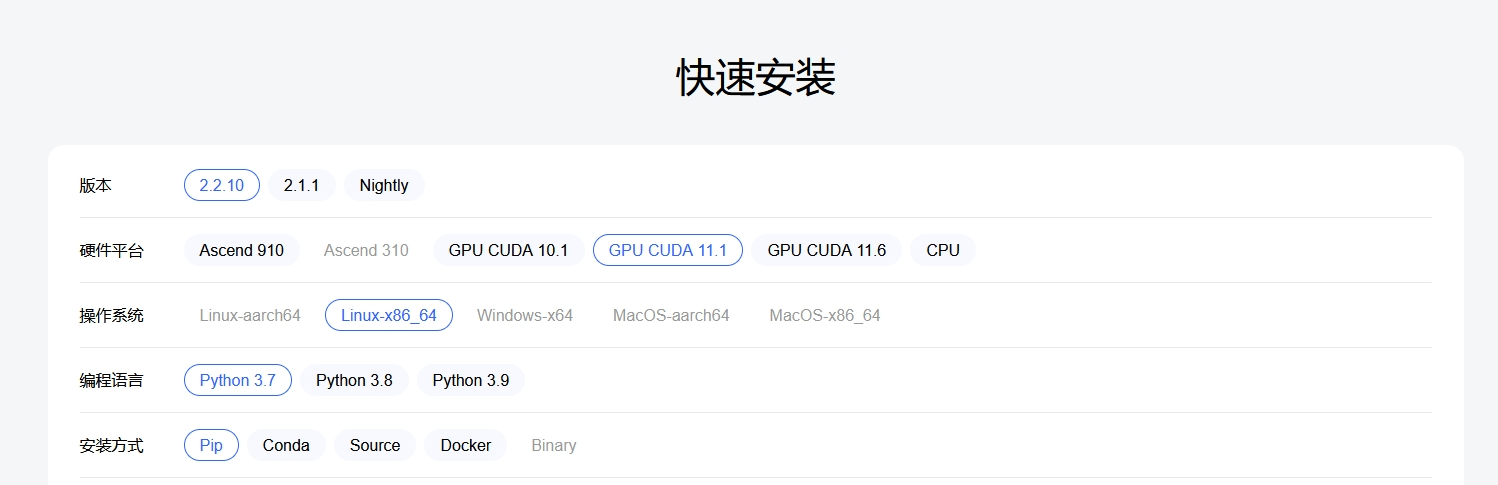
\includegraphics[width=0.8\textwidth]{mindspore.jpg}
  \caption{MindSpore版本对应GPU 、CPU 、NPU的Python版本}
  \label{fig:mindspore}
\end{figure}

这里我们在虚拟环境中创建MindSpore环境,如下所示:
\begin{lstlisting}[language=bash]
conda create -n mindspore_env python=3.8
conda activate mindspore_env
pip install https://ms-release.obs.cn-north-4.myhuaweicloud.com/2.2.10/MindSpore/unified/x86_64/mindspore-2.2.10-cp38-cp38-linux_x86_64.whl --trusted-host ms-release.obs.cn-north-4.myhuaweicloud.com -i https://pypi.tuna.tsinghua.edu.cn/simple
\end{lstlisting}

其它的一些MindSpore教程以及环境搭建可以参考MindSpore官网\footnote{\url{https://www.mindspore.cn/docs/zh-CN/r2.2/index.html}}。

\subsubsection{OneFlow环境安装(选看)}
OneFlow\footnote{\url{https://www.oneflow.org/a/chanpin/oneflow/}}是开源的、采用全新架构设计,世界领先的工业级通用深度学习框架。
OneFlow可以进行分布式训练、多机多卡如单机单卡一样简单;完美契合一站式平台(k8s + docker)、原生支持超大模型;近零运行时开销、线性加速比;灵活支持多种深度学习编译器、自动混合精度;中立开放,合作面广;持续完善的算子集、模型库。 
OneFlow的安装也非常简单,只需要以下的命令即可:
\begin{lstlisting}[language=bash]
conda create -n oneflow_env python=3.8
conda activate oneflow_env
python3 -m pip install -f https://release.oneflow.info oneflow==0.9.0+cu116
\end{lstlisting}

这里我们选择了cu116版本的OneFlow,也可以选择其他版本的OneFlow。
教程以及使用方法参考官方教程\footnote{\url{https://docs.oneflow.org/master/index.html}}即可。

\subsubsection{MXNet环境安装(选看)}
MXNet是一个高效且灵活的开源深度学习框架,由Apache软件基金会支持。
它提供了一个可扩展的计算图模型,允许用户在多种计算设备上运行深度学习模型,包括CPU、GPU和多个机器。
MXNet的设计注重效率和性能,可以处理大规模的数据集和复杂的模型。
它具有用户友好的API,使得构建、训练和部署模型变得简单。
MXNet还提供了丰富的工具和库,用于数据加载、模型评估和可视化。
总之,MXNet是一个功能强大且易于使用的开源框架,适用于各种深度学习任务和应用。

对于Python版本的MXNet,可以通过以下的命令进行安装:
\begin{lstlisting}[language=bash]
conda create -n mxnet_env python=3.8
conda activate mxnet_env
pip install mxnet-cu112
\end{lstlisting}
这里安装的是CUDA11.2版本的MXNet,也可以选择其他版本的MXNet。

使用以下Python代码测试MXNet是否安装成功:
\begin{lstlisting}[language=python]
  import mxnet as mx
  a = mx.nd.ones((2, 3), mx.gpu())
  b = a * 2 + 1
  c = b.asnumpy()
  print(c)
\end{lstlisting}

\subsubsection{Chainer环境安装(选看)}
Chainer是一个开源的深度学习库\footnote{\url{https://chainer.org/}},它提供了一种简单而灵活的方式来构建和训练神经网络模型。
Chainer的特点之一是它采用了动态图计算的方式,这意味着用户可以在模型构建和训练过程中使用Python的控制流和条件语句,使得模型的构建更加灵活和可读性更强。
Chainer还提供了丰富的优化算法和损失函数,以及可视化工具来帮助用户分析和调试模型。同时,Chainer还支持多种硬件加速器,如GPU和FPGA,以加快模型的训练和推理速度。
总之,Chainer是一个功能强大且易于使用的深度学习库,适用于各种机器学习任务。

Chainer的安装非常简单,只需要以下的命令即可:
\begin{lstlisting}[language=bash]
conda create -n chainer_env python=3.8
conda activate chainer_env
pip install chainer
\end{lstlisting}

可以在官方文档\footnote{\url{https://docs.chainer.org/en/stable/}}中看多个例子学会此深度学习库的用法。

\subsubsection{Theano环境安装(选看)}
Theano 是一个开源的机器学习库,它主要用于高效地定义、优化和评估数学表达式。它可以在多种硬件平台上运行,包括CPU和GPU,并且能够自动优化代码以提高性能。
同时提供了一个符号计算框架,其中可以定义各种数学表达式,如张量和矩阵操作。它还提供了许多高级的优化技术,以确保计算过程的高效性和准确性。
Theano 还支持自动求导,这对于训练机器学习模型非常重要。通过定义损失函数并使用Theano的自动求导功能,可以方便地计算梯度并进行模型的参数更新。
Theano 还具有与其他常用机器学习库(如NumPy和SciPy)的良好集成,可以方便地进行数据处理和模型评估。

Theano GPU环境的底层设计主要是依靠pygpu模块进行神经网络的加速。所以第一步首先要安装好pygpu环境。
首先创建一个虚拟环境:
\begin{lstlisting}[language=bash]
conda create -n theano_env python=3.8
conda activate theano_env
\end{lstlisting}

有以下的两种方式进行安装pygpu:
\begin{itemize}
  \item 第一种是在conda环境下安装。直接输入以下的命令就可以进行安装:
\begin{lstlisting}[language=bash]
conda install pygpu
\end{lstlisting}

  这个也在conda-forge包中进行安装
\begin{lstlisting}[language=bash]
conda install -c conda-forge pygpu
\end{lstlisting}
  
  然后再安装theano神经网络库的环境
\begin{lstlisting}[language=bash]
pip install theano   # 或者是 conda install theano
\end{lstlisting}
  \item 第二种方法是通过源码进行安装。
  首先编译libpygpuarray,需要cmake,c99,cython等依赖环境。cython环境可以直接通过pip安装:
\begin{lstlisting}[language=bash]
pip install cython
\end{lstlisting}
  安装cmake可以直接这样安装
\begin{lstlisting}[language=bash]
sudo apt install cmake
\end{lstlisting}
  
  下面是对libpygpuarray进行安装。首先从theano的github上下载libpygpuarray的源码文件:
  \begin{lstlisting}[language=bash]
git clone https://github.com/Theano/libgpuarray.git
cd libgpuarray
  \end{lstlisting}
  创建编译目录进行编译。如果想用libgpuarray进行开发,可以这样有如下编译方法:
\begin{lstlisting}[language=bash]
cd libgpuarray
mkdir Build
cd Build
# you can pass -DCMAKE_INSTALL_PREFIX=/path/to/somewhere to install to an alternate location
cmake .. -DCMAKE_BUILD_TYPE=Release # or Debug if you are investigating a crash
make
make install
cd ..
\end{lstlisting}
  如果只是想安装pygpu,只需要先激活虚拟环境(如果需要的话),然后在源码文件夹下面进行以下操作
  \begin{lstlisting}[language=bash]
python setup.py build
python setup.py install
  \end{lstlisting}
\end{itemize}

Theano文档中描述了很多Theano的使用方法,可以参考Theano官网\footnote{\url{https://docs.huihoo.com/theano/0.9/}}。

\paragraph{theano GPU配置文件的设置}

在用户文件夹下创建.theanorc文件:
\begin{lstlisting}[language=bash]
  nano ~/.theanorc
\end{lstlisting}

并且写入以下的配置文件
\begin{lstlisting}[language=bash]
  [global]
  device = cuda
  floatX=float32
  root = /usr/local/cuda
  [nvcc]
  fastmath=True
  compiler_bindir=/usr/local/cuda-10.1/bin
  [blas]
  ldflags = -lopenblas
  [cuda]
  root = /usr/local/cuda-10.1
  [dnn]
  enabled=True
  inclue_path=/usr/local/cuda/include
  library_path=/usr/local/cuda/lib64
\end{lstlisting}

由于Theano目前已经不再更新,所以尽量使用Docker容器运行Theano环境,这里我列举了CUDA-10.1作为Theano的GPU加速环境。

\paragraph{theano GPU配置文件的测试}

创建以下的python文件
\begin{lstlisting}[language=python]
from theano import function, config, shared, tensor
import numpy
import time
            
vlen = 10 * 30 * 768  # 10 x #cores x # threads per core
iters = 1000

rng = numpy.random.RandomState(22)
x = shared(numpy.asarray(rng.rand(vlen), config.floatX))
f = function([], tensor.exp(x))
print(f.maker.fgraph.toposort())
t0 = time.time()
for i in range(iters):
r = f()
    t1 = time.time()
    print("Looping %d times took %f seconds" % (iters, t1 - t0))
    print("Result is %s" % (r,))
    if numpy.any([isinstance(x.op, tensor.Elemwise) and
    	('GPU' not in type(x.op).__name__) for x in f.maker.fgraph.toposort()]):
print('Used the cpu')
else:
print('Used the gpu')
\end{lstlisting}

显示Used the GPU即配置成功。

\paragraph{关于Theano的一些深度学习库}

\begin{itemize}
  \item deepnet深度学习库
  \item lasagne深度学习库
\end{itemize}

这里注意对一些文件中有个地方的卷积函数进行修改:
import lasagne 的时候发现下列错误:
\begin{lstlisting}[language=bash]
  ImportError: cannot import name 'downsample'
\end{lstlisting}

解决方案如下:
\begin{enumerate}[label=\arabic*). ]
  \item 找到下列发生错误的文件 \verb|\lasagne\layers\pool.py|;
  \item 将其中的 \verb|from theano.tensor.signal import downsample| 修改为
	
  \verb|from theano.tensor.signal.pool import pool_2d|
  \item 将文件中的\verb|downsample.max_pool_2d| 改为  \verb|pool_2d|。
\end{enumerate}

\subsection{Julia深度学习环境配置(选看)}
Julia 是一种高级、动态和高性能的编程语言,主要用于科学计算、数据分析和数值计算。它的设计目标是提供一种易于使用的语言,同时保持与传统科学计算语言(如Matlab和Python)相似的表达能力。

Julia 的特点之一是它的速度,它具有接近于传统编译语言(如C、C++)的性能。这得益于 Julia 的即时编译(JIT)技术,它能够将代码实时编译为机器码,从而提供高效的执行。此外,Julia 还支持多线程和并行计算,使得它在处理大规模数据和复杂计算任务时表现出色。

Julia 的语法简洁、灵活,易于学习和使用。它支持面向对象和函数式编程,并提供了丰富的内置函数和库,用于处理数值计算、线性代数、统计分析、优化等任务。此外,Julia 还具有强大的数据处理能力,可以直接操作数组、矩阵和其他数据结构。

Julia 是一个开源项目,拥有活跃的社区支持。它可以在多个操作系统上运行,并且可以与其他编程语言(如Python、C、R)进行无缝集成,使得它成为科学计算和数据分析领域的一种强大工具。
所以在深度学习环境中,Julia也是一个非常好的选择。
\subsubsection{Julia环境安装}

\subsubsection{Flux ML 安装}
\subsubsection{其他一些包环境}
\subsection{Rust深度学习环境配置(选看)}
\subsubsection{Rust环境安装}
\subsubsection{Candle深度学习环境安装}
\subsubsection{Burn深度学习环境安装}
Burn\footnote{\url{https://github.com/tracel-ai/burn}}是一个基于Rust语言的深度学习库。
\subsubsection{Tch-rs深度学习环境安装}
\subsubsection{Neuronika深度学习环境}
https://github.com/neuronika/neuronika
\subsubsection{其他一些包环境}
\subsection{Go深度学习环境配置(选看)}
\subsubsection{Go语言环境安装}
\subsubsection{Gorgonia深度学习环境安装}
\subsection{lua深度学习环境配置(选看)}
\subsubsection{torch7深度学习环境安装}
Torch7是一种用于深度学习的开源框架,它基于Lua编程语言。
它提供了一个强大且灵活的工具集合,用于构建和训练深度神经网络模型。
Torch7具有高效的计算能力和易于使用的接口,使得模型的开发和实验变得更加简单。
它支持各种常见的深度学习任务,包括图像分类、目标检测、语音识别等。
此外,Torch7还提供了丰富的扩展库,使得用户可以方便地进行数据处理、可视化和模型优化。
在后续开发中,facebook将Torch7开发转为PyTorch,torch7 也不再进行开发。
总之,Torch7是一个功能强大且易于使用的深度学习框架,适用于各种深度学习应用。
\paragraph{torch7环境安装:}
以Ubuntu系统为例子,首先安装一些编译工具和依赖包:
\begin{lstlisting}[language=bash]
sudo apt-get install gcc g++ git cmake libreadline-dev 
\end{lstlisting}

接下来,我们开始安装torch7环境。
CUDA10.0 以下的环境安装选择:
\begin{lstlisting}[language=bash]
  git clone https://github.com/torch/distro.git ~/torch --recursive
\end{lstlisting}

CUDA10.0 以上的环境安装选择:
\begin{lstlisting}[language=bash]
  git clone https://github.com/nagadomi/distro ~/torch --recursive
\end{lstlisting}

目前在CUDA 11.x环境编译torch7会出现错误。

然后进入torch目录,执行以下的命令:
\begin{lstlisting}[language=bash]
  cd torch
  bash install-deps # 检查并且安装一些依赖项环境
\end{lstlisting}

下一步对torch7进行编译安装:
\begin{lstlisting}[language=bash]
  bash install.sh
\end{lstlisting}

编译完成之后,需要对环境变量进行配置,会有以下的询问,选择yes:
\begin{lstlisting}[language=bash]
Do you want to automatically prepend the Torch install location to PATH and LD_LIBRARY in your /home/asus/.bashrc?(yes/no)
[yes] >>>
yes
\end{lstlisting}

通过以下的命令使得环境变量生效:
\begin{lstlisting}[language=bash]
  source ~/.bashrc
\end{lstlisting}

最后,我们可以通过输入th命令测试torch7环境是否安装成功,如图\ref{fig:torch7_terminal}:
\begin{figure}[hbpt]
  \centering
  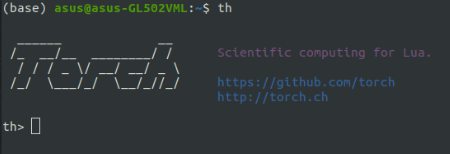
\includegraphics[width=0.8\textwidth]{torch7.png}
  \caption{Torch7命令行界面}
  \label{fig:torch7_terminal}
\end{figure}

在调用torch.inverse(tensor)过程中,出现了一个问题,即getrf : Lapack library not found in compile time。
出现这个问题的主要原因是由于没有安装openBLAS库。
openBLAS库是一个基于C和fortran的矩阵运算库,可以加速矩阵运算。
首先确定操作系统中必须有gfortran编译环境。编译openBLAS需要较低版本的gfortran变异环境。如果没有,则以下命令进行安装:
\begin{lstlisting}[language=bash]
  sudo apt-get install gfortran
\end{lstlisting}

对于Ubuntu22.04操作系统,只有最低版本的gfortran-8,所以安装了gfortran-8版本:
\begin{lstlisting}[language=bash]
  apt-get search gfortran
  sudo apt-get install gfortran-8
  sudo mv /usr/bin/gfortran /usr/bin/gfortran.bak	#进行备份处理
  sudo ln -s gfortran gfortran-8	#进行软链接操作 
\end{lstlisting}

接下来安装openBLAS:

\begin{lstlisting}[language=bash]
  git clone https://github.com/xianyi/OpenBLAS.git
  cd ~/OpenBLAS
  make NO_AFFINITY=1 USE_OPENMP=1 -j4
  sudo make PREFIX=/usr/local/OpenBLAS install  #默认是/opt/OpenBLAS.
  sudo ln -s /opt/OpenBLAS/lib/libopenblas.so.0   /usr/lib/libopenblas.so.0
\end{lstlisting}

安装成功后,设置一下路径
\begin{lstlisting}[language=bash]
  CMAKE_LIBRARY_PATH=/usr/local/OpenBLAS/include:/usr/local/OpenBLAS/lib:$CMAKE_LIBRARY_PATH
  # 或者是在bashrc文件中定义变量CMAKE_LIBRARY_PATH,或者是在安装torch之前定义此变量值
\end{lstlisting}

然后再进行torch的编译安装。

\subsubsection{其他一些包环境}
Lua语言中有一个包管理器luarocks,可以通过luarocks安装一些必要的包。
目前可以需要安装的包有以下几个:
\begin{itemize}
  \item \textbf{gplots:}数据可视化包;
  \item \textbf{nn:}神经网络包;
  \item \textbf{cunn:}CUDA神经网络加速包;
  \item \textbf{cutorch:}CUDA神经网络加速包;
  \item \textbf{cudnn:}CUDA神经网络加速包;
  \item \textbf{iTorch:}Jupyter Notebook的Lua版本。
\end{itemize}

上述的安装方式均可以用luarocks进行安装,如下所示:
\begin{lstlisting}[language=bash]
  luarocks install gplots 
\end{lstlisting}

其他包的安装方式同上述类似。

\subsection{Java深度学习环境配置(选看)}
\subsubsection{Java以及Maven环境安装}
\subsubsection{TensorFlow在Android上的使用}
\subsubsection{Pytorch在Android上的使用}
\subsubsection{DeepLearning4j深度学习环境安装}
\subsubsection{其他一些环境}
\section{远程登录工具使用}
\subsection{公网远程连接桌面工具}
公网远程桌面连接工具有很多,我们这里列举几种较为常见的桌面连接工具。
\begin{itemize}
  \item \textbf{ToDesk\footnote{\url{https://www.todesk.com/download.html}}:}ToDesk远程控制软件是一款稳定流畅的远程控制电脑手机连接软件,可远程桌面办公,远程协助运维.采用端对端加密,让每一次远程访问都安全可靠。
  
  对于Linux 安装方式,选择对应的架构和安装包下载安装即可。我们这里对应的是amd64(x86-64)架构,所以选择对应的Debian/Ubuntu/Mint的deb包进行安装。
  \begin{lstlisting}[language=bash]
    wget https://newdl.todesk.com/linux/todesk-v4.3.1.0-amd64.deb
    sudo dpkg -i todesk-v4.3.1.0-amd64.deb
  \end{lstlisting}

  当然对于Fedora操作系统来说,可以选择对应的rpm包进行安装。
  \begin{lstlisting}[language=bash]
    wget https://newdl.todesk.com/linux/todesk-v4.3.1.0-x86_64.rpm
    sudo rpm -ivh todesk-v4.3.1.0-x86_64.rpm
  \end{lstlisting}
  \item \textbf{向日葵:}向日葵远程控制软件是一款拥有多年远控技术经验的远程控制软件,可远程控制手机,远程桌面连接,远程开机,远程管理等,并深入各行各业提供企业远程办公、企业IT运维、技术支持等企业远程解决方案。
  
  对于Linux 安装方式,选择对应的架构和安装包下载安装即可。这里我们选择Ubuntu/Deepin的amd64(x86-64)架构安装。
  \begin{lstlisting}[language=bash]
    wget https://down.oray.com/sunlogin/linux/SunloginClient_11.0.1.44968_amd64.deb
    sudo dpkg -i sunloginclient_11.0.1.44968_amd64.deb
  \end{lstlisting}
  
  对于Fedora系列的操作系统,选择对应的rpm包进行安装。
  \begin{lstlisting}[language=bash]
    wget https://down.oray.com/sunlogin/linux/SunloginClient_11.0.1.44968_amd64.rpm
    sudo rpm -ivh SunloginClient_11.0.1.44968_x86_64.rpm
  \end{lstlisting}

  Linux系统可能会出现以下依赖包缺少情形,并通过对应的安装命令安装即可
  \begin{itemize}
    \item "libXss.so"依赖包缺少:
    \begin{lstlisting}[language=bash]
      sudo apt-get install libxss1 # Debian系
      sudo yum install libXScrnSaver # Fedora系
    \end{lstlisting}
    \item "webkitgtk3"依赖包缺少:
    \begin{lstlisting}[language=bash]
      sudo apt-get install libwebkitgtk-3.0-0 # Debian系
      sudo yum install libappindicator-gtk3 # Fedora系
    \end{lstlisting}
  \end{itemize}
  
  \item \textbf{RustDesk}
  RustDesk\footnote{\url{https://rustdesk.com/zh/}}是一款开源的远程桌面软件,它是由Rust语言开发的,所以它的运行效率非常高,同时它也是跨平台的远程桌面软件,支持Windows、Linux、MacOS等操作系统。
  RustDesk可以有效代替TeamViewer、向日葵、AnyDesk等远程桌面软件,它的安装也非常简单,只需要下载对应的安装包即可。
  下载地址是Github地址\footnote{\url{https://github.com/rustdesk/rustdesk/releases}},从发行版中选择自己的合适的架构和操作系统,这里我们选择Debian系的x86-64.deb包。
  安装如下所示
  \begin{lstlisting}[language=bash]
    wget https://github.com/rustdesk/rustdesk/releases/download/1.2.3/rustdesk-1.2.3-x86_64.deb
    sudo dpkg -i rustdesk-1.2.3-x86_64.deb
  \end{lstlisting}
  
  对于Fedora系列的操作系统安装步骤如下所示
  \begin{lstlisting}[language=bash]
    wget https://github.com/rustdesk/rustdesk/releases/download/1.2.3/rustdesk-1.2.3-0.x86_64.rpm
    sudo rpm -ivh rustdesk-1.2.3-0.x86_64.rpm
  \end{lstlisting}
  服务器端安装成功之后,可以设置自己的密码,在客户端安装对应的RustDesk,然后就可以远程操控电脑了。
  \item \textbf{AnyDesk(选看)}
  AnyDesk\footnote{\url{}}是一种远程桌面控制软件,它允许你远程访问电脑,或与其他人远程协作。通过AnyDesk,你可以直接从你的电脑连接到另一台电脑,并在其上执行各种操作。
  AnyDesk具有高度安全性和相对较快的连接速度,支持跨平台,包括Windows,Mac OS,Android和iOS。而且AnyDesk支持多语言设置,你可以用你想用的语言来使用AnyDesk。
  安装方式有两种,一种是基于源安装的方式,添加一下的源
  \begin{lstlisting}[language=bash]
    wget -qO - https://keys.anydesk.com/repos/DEB-GPG-KEY | sudo apt-key add -
    echo "deb http://deb.anydesk.com/ all main" > /etc/apt/sources.list.d/anydesk-stable.list
    sudo apt update
    sudo apt install anydesk
  \end{lstlisting}
  这样就可以使用AnyDesk了。如果是rpm系列的包方式(Fedora系列、SUES系列等),可以查看官方源\footnote{\url{http://rpm.anydesk.com/howto.html}}导入方式。
  另外一种是基于二进制包的安装方式,安装方式如下所示
  \begin{lstlisting}[language=bash]
    wget https://download.anydesk.com/linux/anydesk_6.1.1-1_amd64.deb
    sudo dpkg -i anydesk_6.1.1-1_amd64.deb
  \end{lstlisting}
  对于RPM系列的操作系统,安装方式如下所示
  \begin{lstlisting}[language=bash]
    wget https://download.anydesk.com/linux/anydesk-6.1.1-1.x86_64.rpm
    sudo rpm -ivh anydesk-6.1.1-1.x86_64.rpm
  \end{lstlisting}
  \end{itemize}
\subsection{文件传输工具}
文件传输工具首选的是FileZilla\footnote{\url{https://filezilla-project.org/download.php}},它是一个开源的FTP工具,可以在Windows、Linux、MacOS等操作系统上运行。
它支持FTP、FTPS和SFTP协议,可以在客户端和服务器之间传输文件,并且支持IPv6,可以在IPv6网络上运行。
选择对应的操作系统以及处理器架构即可以安装,打开之后界面如图\ref{fig:filezilla}所示:

\begin{figure}[hbpt]
  \centering
  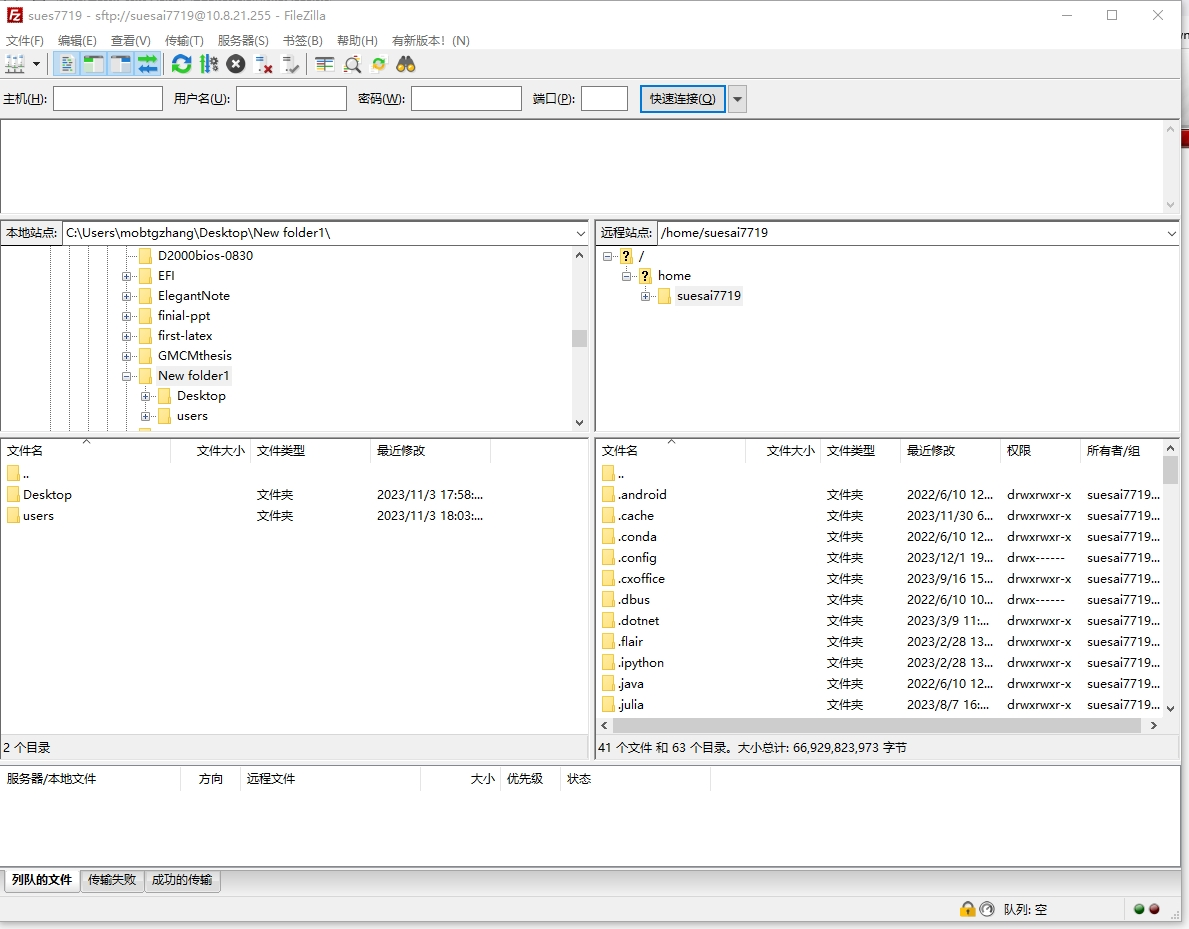
\includegraphics[width=0.8\textwidth]{filezilla.jpg}
  \caption{FileZilla界面}
  \label{fig:filezilla}
\end{figure}

\newpage
\subsection{VSCode配置SSH远程连接}
安装VSCode\footnote{\url{https://code.visualstudio.com/}}之后,打开本地的VSCode开发插件菜单,在扩展程序中搜素Remote-SSH并安装,如图\ref{fig:vscode}所示。

\begin{figure}[hbpt]
  \centering
  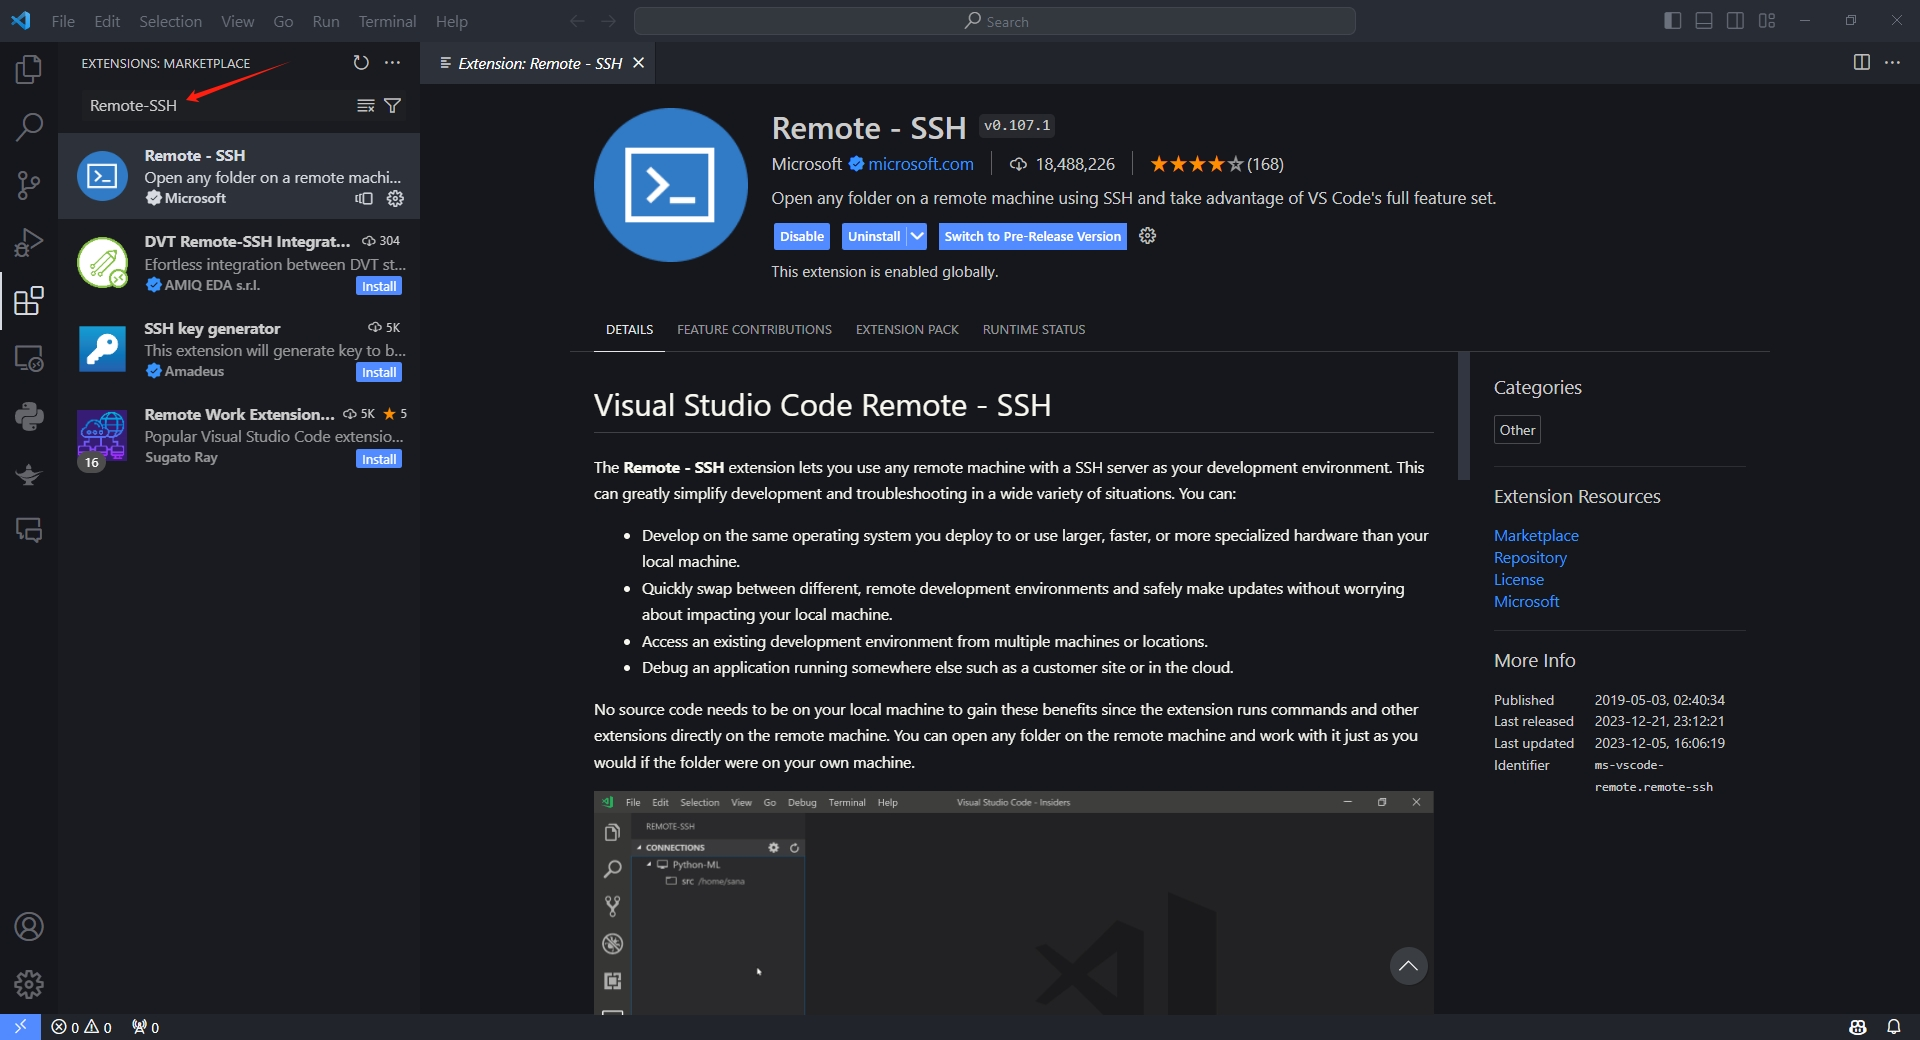
\includegraphics[width=0.8\textwidth]{vscode.jpg}
  \caption{VSCode界面}
  \label{fig:vscode}
\end{figure}

按照图示进行点击,完成添加SSH主机。
\begin{figure}[hbpt]
  \centering
  \subfloat[找到主机连接面板]{
    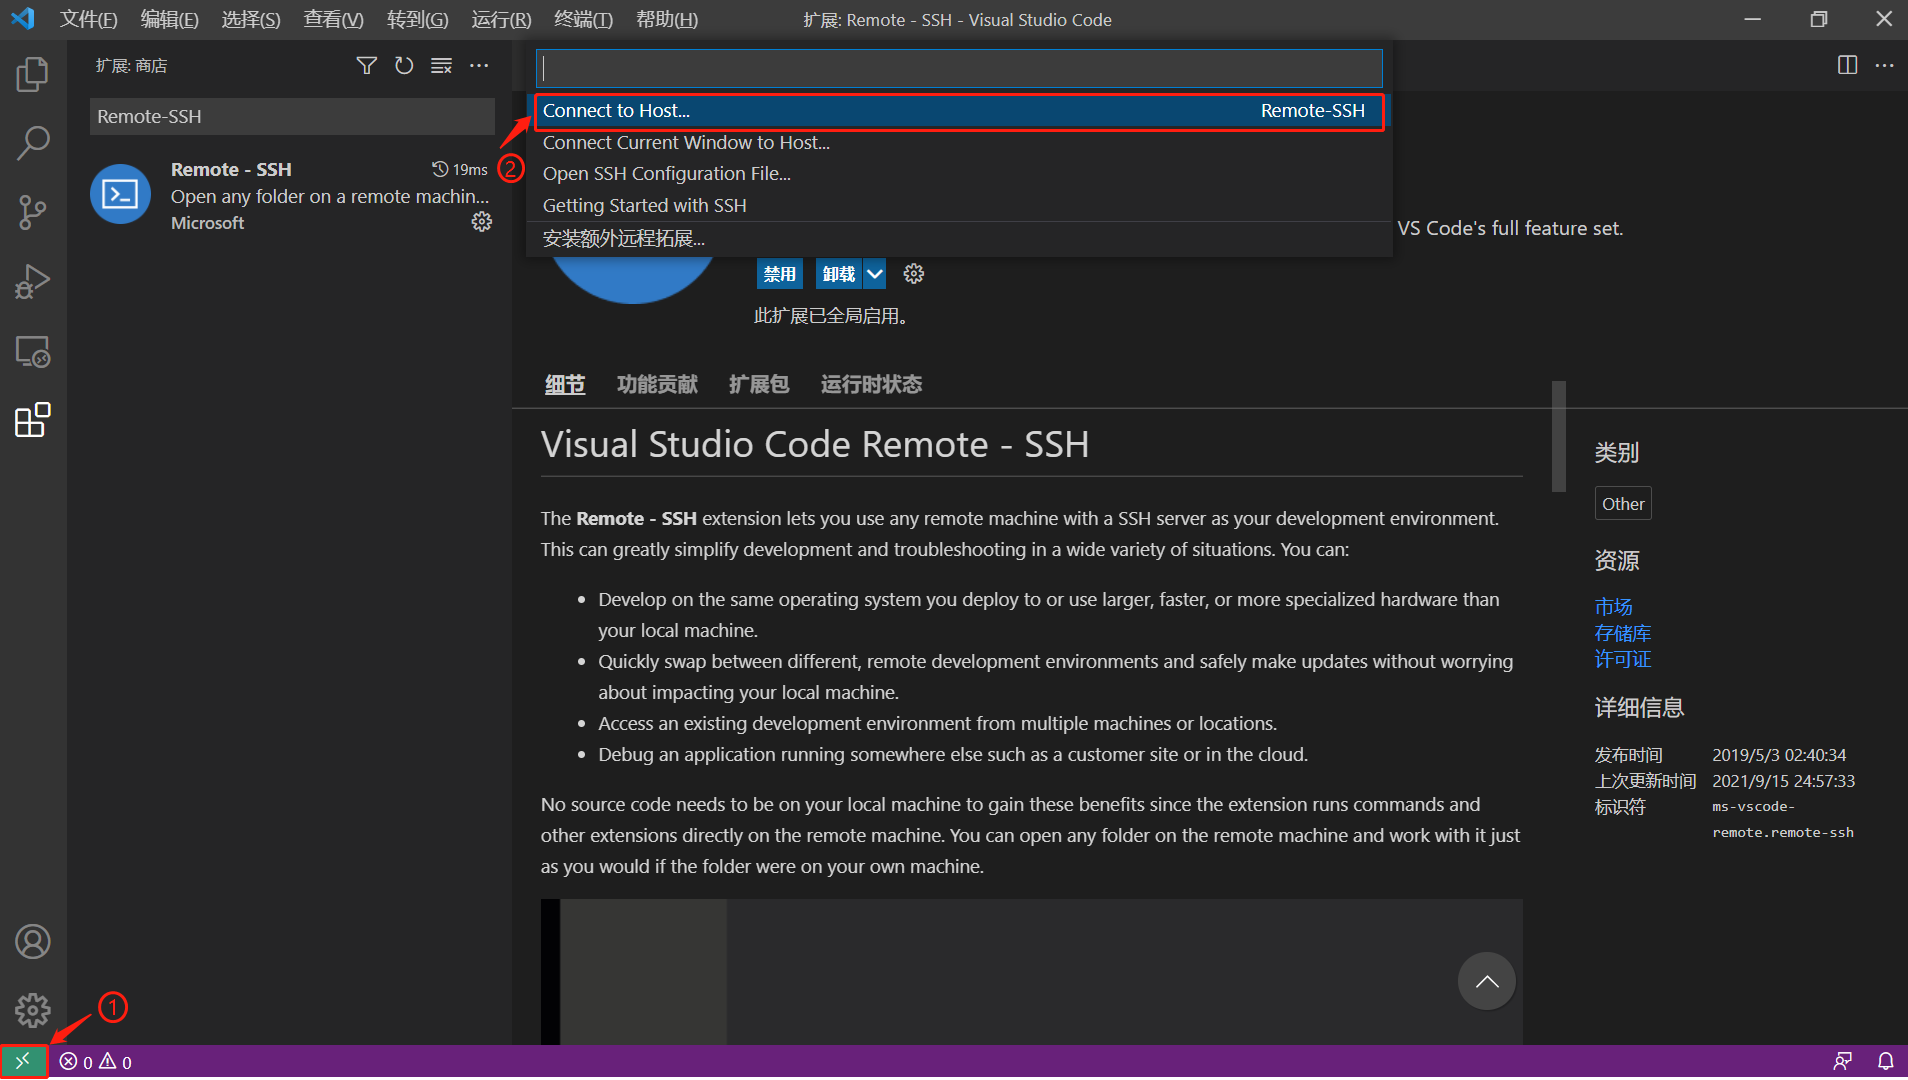
\includegraphics[width=0.8\textwidth]{vscode2.png}
  }
  \quad
  \subfloat[找到连接IP地址]{
    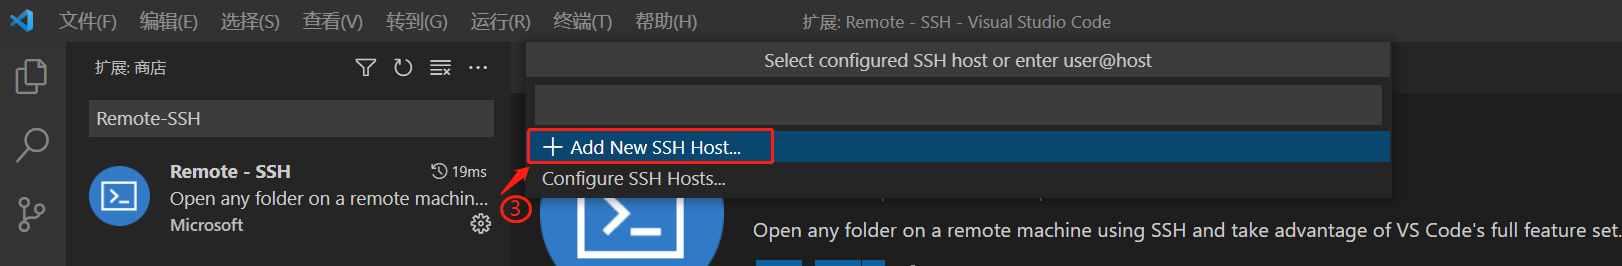
\includegraphics[width=0.8\textwidth]{vscode3.png}
  }
  \caption{VSCode添加SSH主机}
  \label{fig:vscode2}
\end{figure}

添加登录的命令,例如登录命令为
\begin{lstlisting}[language=bash]
  ssh -p ip_port username@ip_address
\end{lstlisting}

ip\_port 为SSH端口号,默认为22,username为用户名,ip\_address为IP地址。

回车后会弹出以下自定义SSH config 文件的弹窗,不需要修改,直接回车即可。
选择直接回车即可。马上可能会弹出选择远程服务器是Windows、Linux和Mac系统的选项,请选择Linux。

然后就可以像在自己PC机上一样使用VSCode进行远程开发了。
\begin{figure}
  \centering
  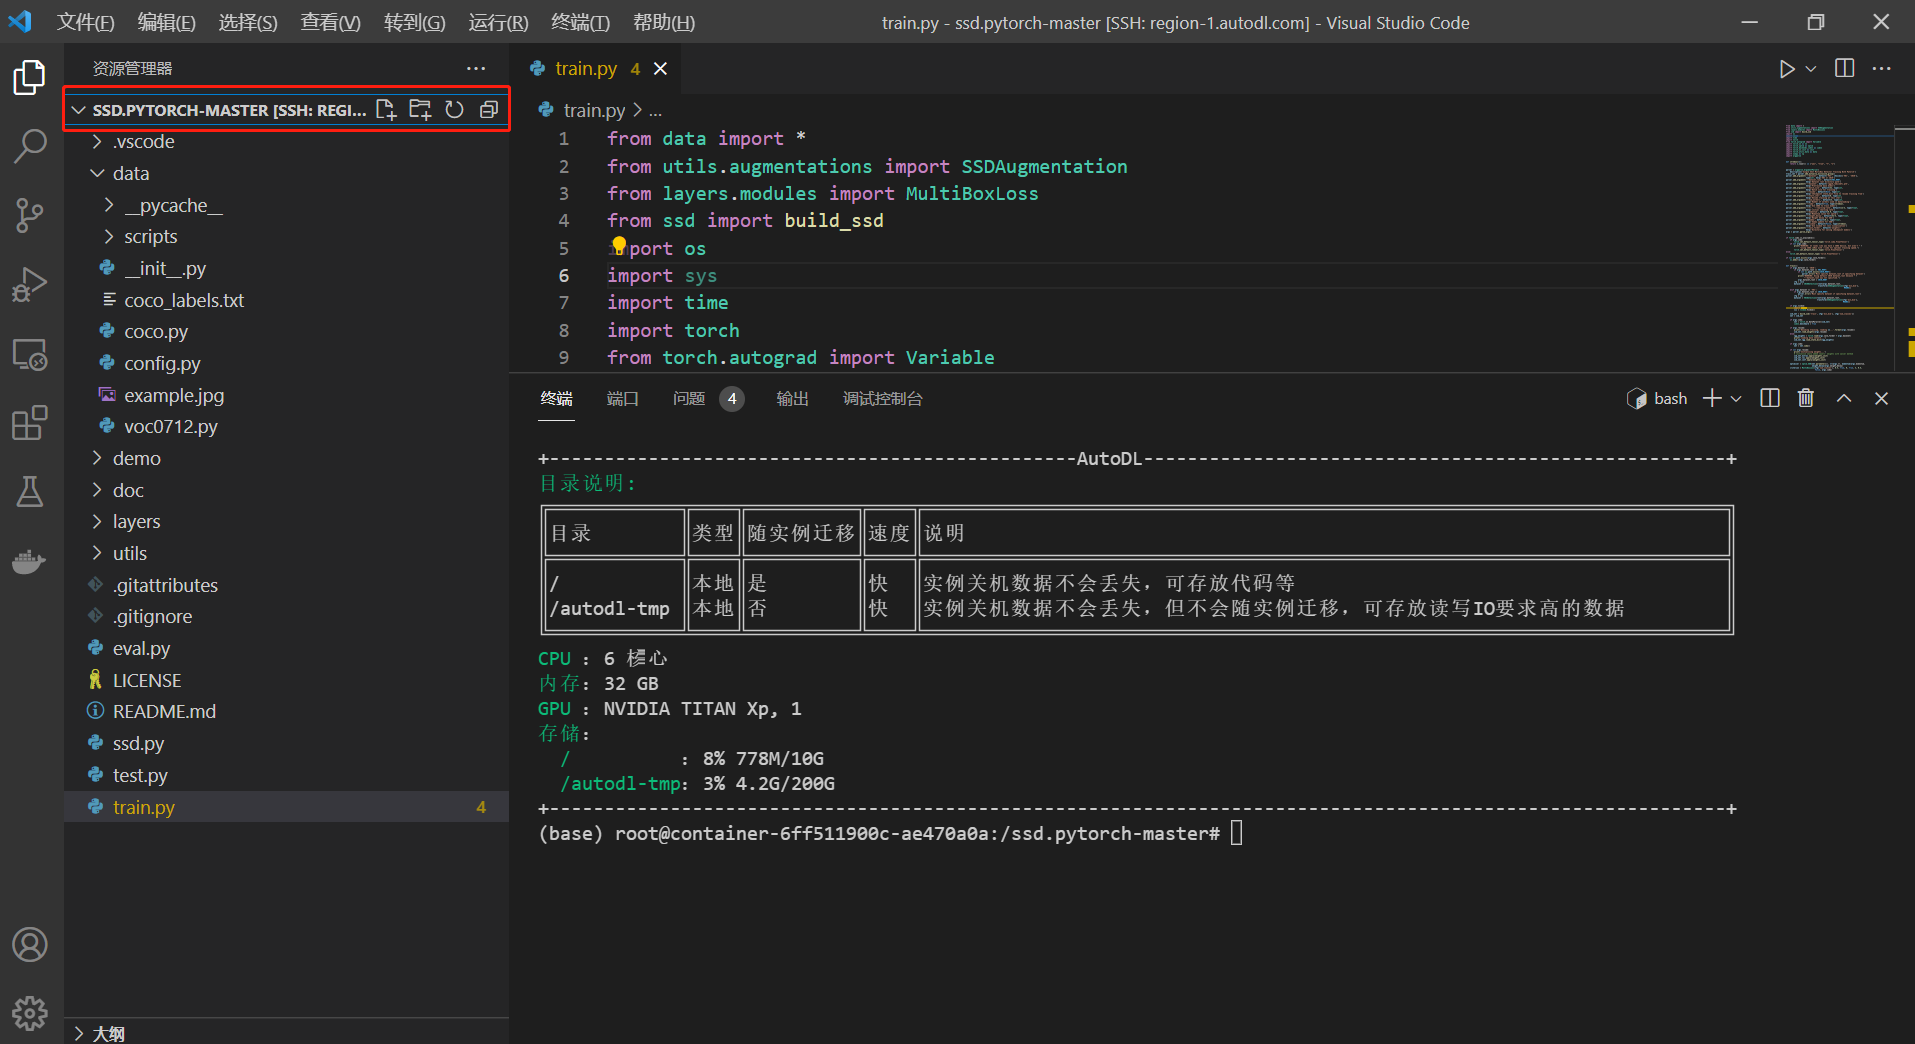
\includegraphics[width=0.65\textwidth]{vscode4.png}
  \caption{VSCode远程开发}
  \label{fig:vscode4}
\end{figure}

\newpage
\subsection{PyCharm配置SSH远程连接}
确认您安装的PyCharm是社区版还是专业版,只有专业版才支持远程开发功能。

\textbf{配置PyCharm:}[File] -> [Settings],打开以下设置弹窗,搜索interpreter找到[Python interpreter]设置项;
\begin{figure}[hbpt]
  \centering
  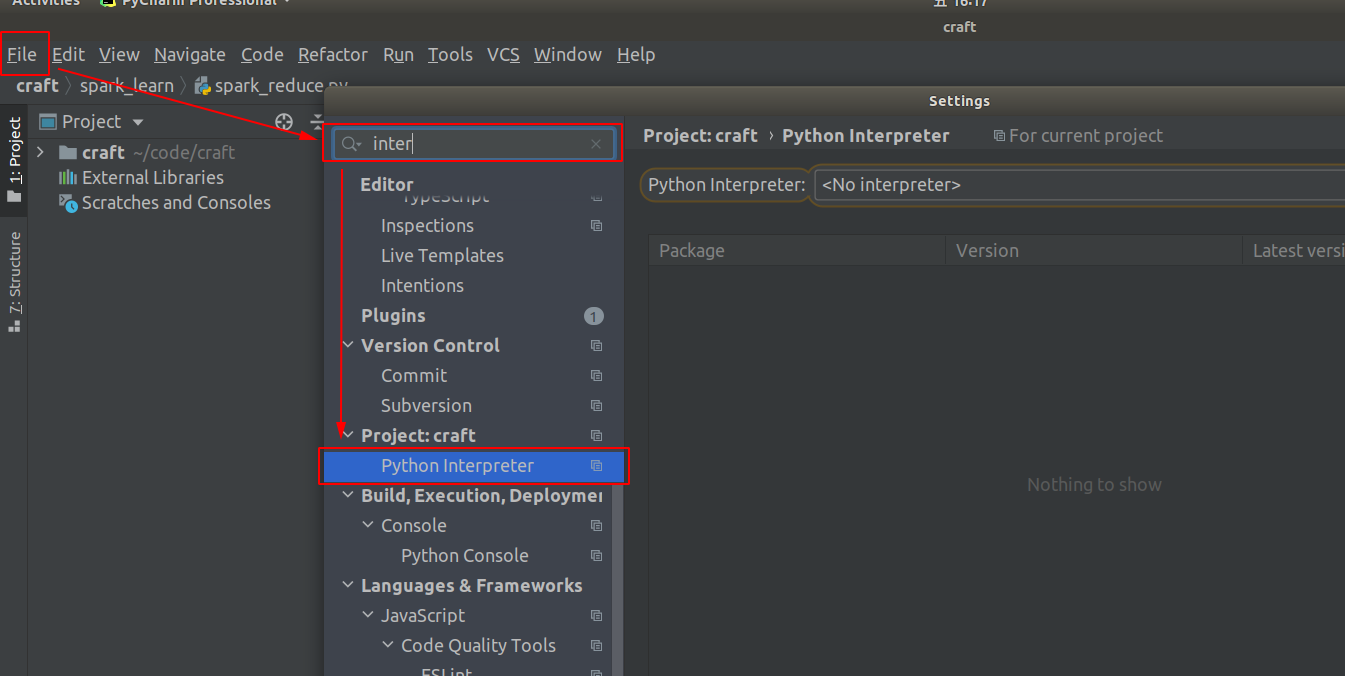
\includegraphics[width=0.8\textwidth]{pycharm1.png}
  \caption{PyCharm设置}
  \label{fig:pycharm1}
\end{figure}

点击Add Interpreter,选择On SSH并点击 (PyCharm社区版本无该选项)
\begin{figure}[hbpt]
  \centering
  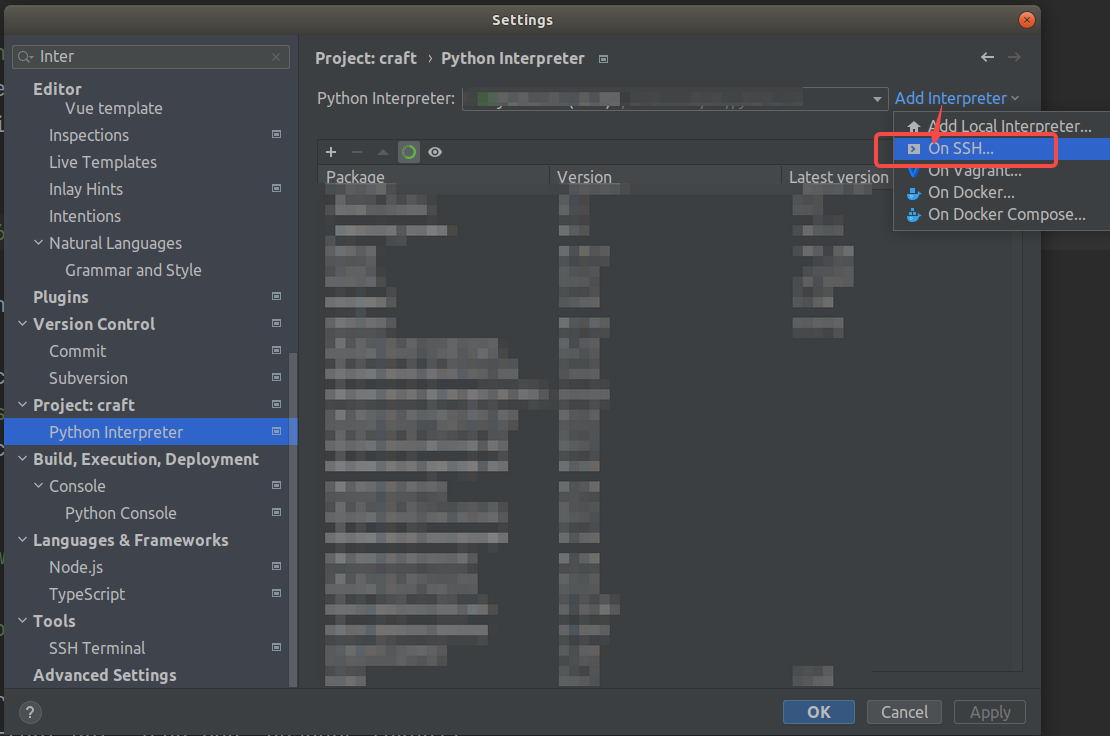
\includegraphics[width=0.8\textwidth]{pycharm2.png}
  \caption{PyCharm设置}
  \label{fig:pycharm2}
\end{figure}

将实例SSH指令中的Host、Port与Username进行匹配和填写,然后输入密码。
\begin{figure}[hbpt]
  \centering
  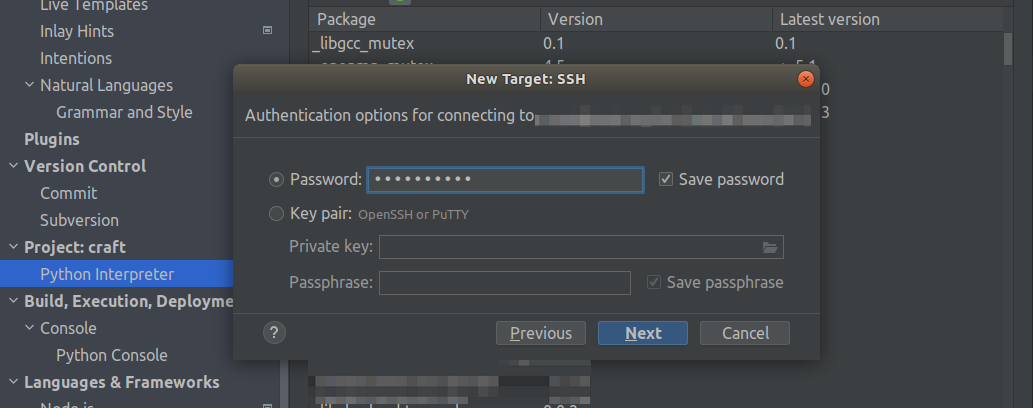
\includegraphics[width=0.8\textwidth]{pycharm3.png}
  \caption{PyCharm设置}
  \label{fig:pycharm3}
\end{figure}

\newpage
继续下一步,选择System Interpreter,Python或虚拟环境则根据实际情况填写。
配置同步目录,意思是本地项目和远程实例中的哪个目录进行关联。
\begin{figure}[hbpt]
  \centering
  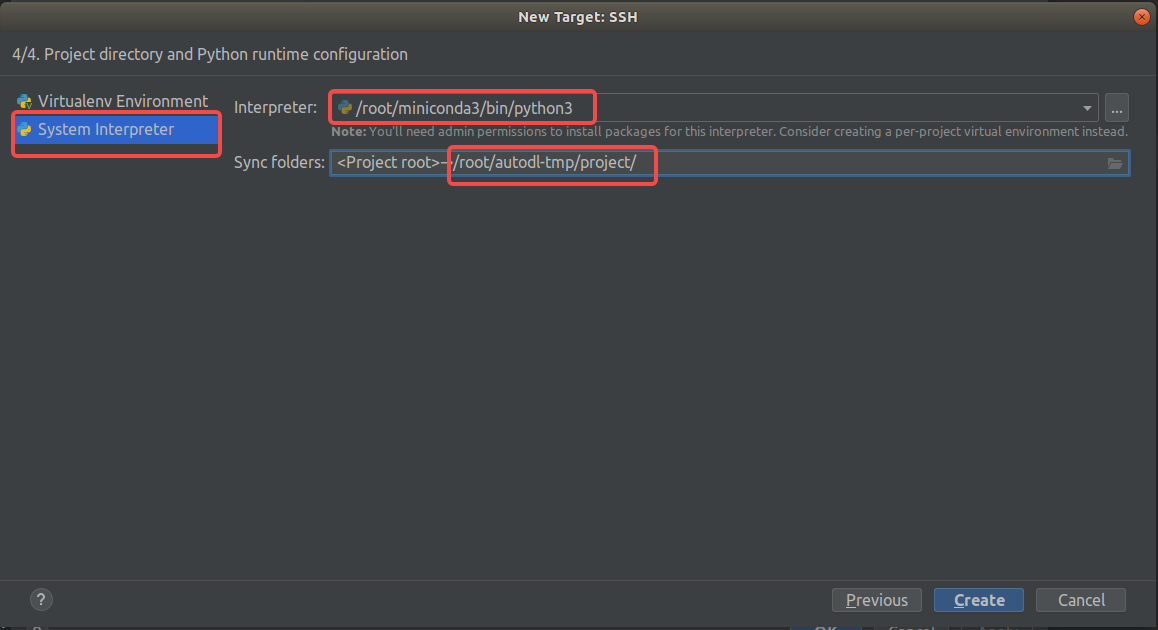
\includegraphics[width=0.8\textwidth]{pycharm4.png}
  \caption{PyCharm设置}
  \label{fig:pycharm4}
\end{figure}

如果您在运行时找不到Python文件,可能是没有自动同步代码,那么可以选择手动同步:
\begin{figure}[hbpt]
  \centering
  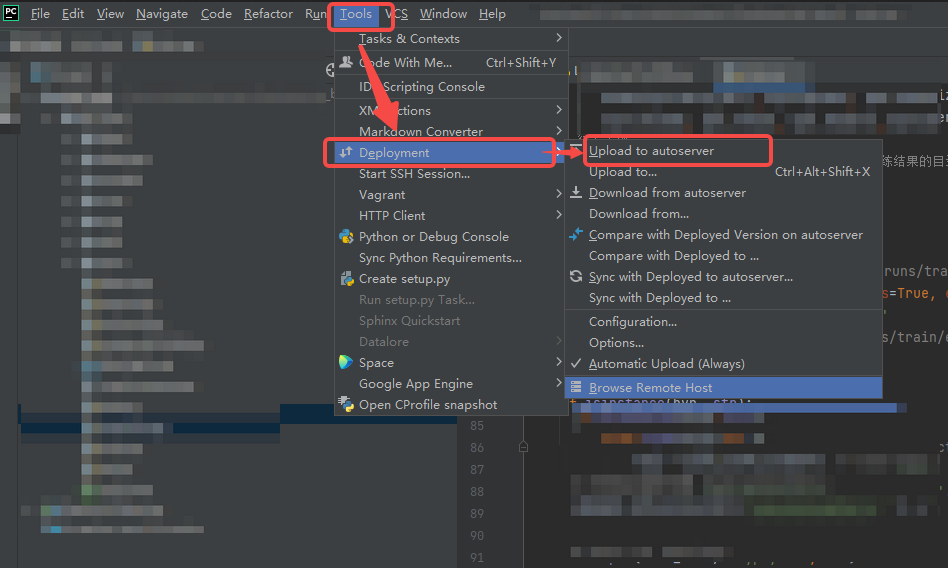
\includegraphics[width=0.8\textwidth]{pycharm6.png}
  \caption{PyCharm设置}
  \label{fig:pycharm6}
\end{figure}

\newpage
配置好PyCharm远程开发后,可以在PyCharm的终端中下拉找到远程服务器打开远程终端:
\begin{figure}[hbpt]
  \centering
  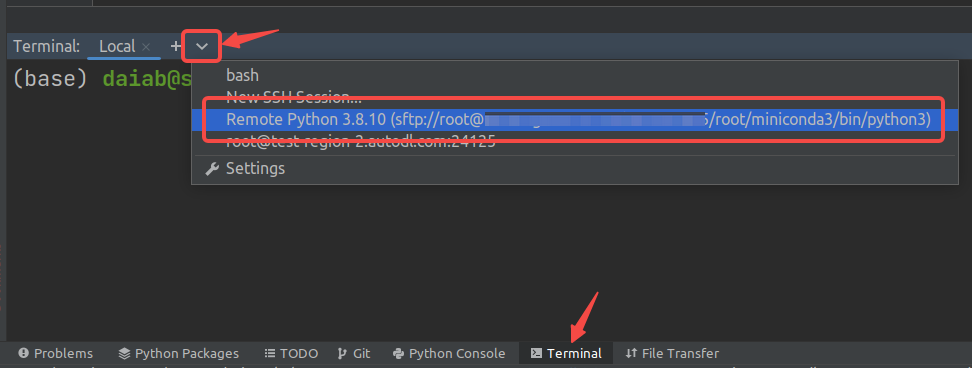
\includegraphics[width=0.8\textwidth]{pycharm5.png}
  \caption{PyCharm设置}
  \label{fig:pycharm5}
\end{figure}

也可以查看官方教程进行配置\footnote{\url{https://www.jetbrains.com/help/pycharm/configuring-remote-interpreters-via-ssh.html}}。

\subsection{内网穿透(选看)}
\section{Docker 使用方法}
Docker\footnote{\url{https://www.docker.com/}}是一种开源的容器化平台,它可以帮助开发人员和运维团队更高效地构建、打包、分发和运行应用程序。
Docker使用轻量级的容器技术,将应用程序及其依赖项打包到一个可移植的容器中,使应用程序可以在任何环境中运行。
通过使用Docker,开发人员可以快速部署应用程序,减少环境配置和依赖项管理的复杂性。
Docker还提供了强大的容器管理工具,使运维团队能够轻松地管理和扩展容器化的应用程序。
\subsection{Docker安装}
对于Ubuntu22.04 可以通过以下的方式安装Docker,首先卸载与Docker冲突的软件包
\begin{lstlisting}[language=bash]
  for pkg in docker.io docker-doc docker-compose docker-compose-v2 podman-docker containerd runc;
  do 
    sudo apt-get remove $pkg;
  done
\end{lstlisting}

有两种安装方式,一种是基于源安装的方式,另外是一种是基于二进制包的安装方式。
\paragraph{基于apt源安装的方式}
通过以下的方式添加docker源:
\begin{lstlisting}[language=bash]
  # 添加Docker的官方GPG公钥:
  sudo apt-get update
  sudo apt-get install ca-certificates curl gnupg
  sudo install -m 0755 -d /etc/apt/keyrings
  curl -fsSL https://download.docker.com/linux/ubuntu/gpg | sudo gpg --dearmor -o /etc/apt/keyrings/docker.gpg
  sudo chmod a+r /etc/apt/keyrings/docker.gpg
  
  # 添加apt源:
  echo \
    "deb [arch=$(dpkg --print-architecture) signed-by=/etc/apt/keyrings/docker.gpg] https://download.docker.com/linux/ubuntu \
    $(. /etc/os-release && echo "$VERSION_CODENAME") stable" | \
    sudo tee /etc/apt/sources.list.d/docker.list > /dev/null
  sudo apt-get update
\end{lstlisting}

然后我们直接添加Docker的最新版本的源即可,按照以下的命令进行安装:
\begin{lstlisting}[language=bash]
  sudo apt-get install docker-ce docker-ce-cli containerd.io docker-buildx-plugin docker-compose-plugin
\end{lstlisting}

用下面的命令可以验证Docker是否安装成功:
\begin{lstlisting}[language=bash]
  sudo docker run hello-world
\end{lstlisting}

\paragraph{基于二进制包安装的方式}
如果你不能使用Docker的apt存储库来安装Docker引擎,可以通过下载发布的deb文件并手动安装。
每次升级Docker引擎时,都需要下载一个新文件,安装步骤如下所示:
\begin{enumerate}[label=(\arabic*). ]
  \item 打开Docker官方下载页面网址\footnote{\url{https://download.docker.com/linux/ubuntu/dists/}};
  \item 选择Ubuntu版本,这里我们选择Ubuntu22.04版本;
  \item 到pool/stable/ 文件夹下,由于我们服务器处理器为x86-64架构,所以这里选择amd64作为安装包文件;
  \item 下载Docker Engine、CLI、containerd和Docker Compose包的以下deb文件;
  \begin{itemize}
    \item \verb|containerd.io_<version>_<arch>.deb|;
    \item \verb|docker-ce_<version>_<arch>.deb|;
    \item \verb|docker-ce-cli_<version>_<arch>.deb|;
    \item \verb|docker-buildx-plugin_<version>_<arch>.deb|;
    \item \verb|docker-compose-plugin_<version>_<arch>.deb|
  \end{itemize}
  安装.deb包,将以下示例中的路径更新为下载Docker软件包的位置。
  \begin{lstlisting}[language=bash]
    sudo dpkg -i ./containerd.io_<version>_<arch>.deb \
      ./docker-ce_<version>_<arch>.deb \
      ./docker-ce-cli_<version>_<arch>.deb \
      ./docker-buildx-plugin_<version>_<arch>.deb \
      ./docker-compose-plugin_<version>_<arch>.deb
  \end{lstlisting}
  Docker守护进程会自动启动。
  通过运行helloworld映像验证Docker引擎安装是否成功。
  \begin{lstlisting}[language=bash]
    sudo service docker start
    sudo docker run hello-world
  \end{lstlisting}
  此命令下载测试映像并在容器中运行。
  当容器运行时,它会打印一条确认消息并退出。
\end{enumerate}

\paragraph{NVIDIA Docker安装}
NVIDIA Docker\footnote{\url{https://docs.nvidia.com/datacenter/cloud-native/container-toolkit/latest/index.html}}是一个开源的项目,它可以让用户在Docker容器中运行GPU应用程序。
NVIDIA Docker包括一个运行时库和一个Docker命令行实用程序。
NVIDIA Docker运行时库是一个动态库,它提供了一个Docker API的实现,该实现可以将Docker容器中的GPU设备映射到主机上的NVIDIA设备。

通过下面的方法可以添加对应的apt源:
\begin{lstlisting}[language=bash]
  curl -fsSL https://nvidia.github.io/libnvidia-container/gpgkey | sudo gpg --dearmor -o /usr/share/keyrings/nvidia-container-toolkit-keyring.gpg \
  && curl -s -L https://nvidia.github.io/libnvidia-container/stable/deb/nvidia-container-toolkit.list | \
    sed 's#deb https://#deb [signed-by=/usr/share/keyrings/nvidia-container-toolkit-keyring.gpg] https://#g' | \
    sudo tee /etc/apt/sources.list.d/nvidia-container-toolkit.list
\end{lstlisting}

更显源,并安装NVIDIA Container Toolkit
\begin{lstlisting}[language=bash]
  sudo apt-get update
  sudo apt-get install -y nvidia-container-toolkit
  sudo systemctl restart docker
\end{lstlisting}

这样就安装好了对应的NVIDIA Docker。


\paragraph{Docker镜像加速}
国内从DockerHub拉取镜像有时会遇到困难,此时可以配置镜像加速器。
Docker官方和国内很多云服务商都提供了国内加速器服务,建议根据运行docker的云平台选择对应的镜像加速服务。
下面列出国内常用的加速站点,排名不分先后,总体来说阿里云速度较稳定。
\begin{itemize}
  \item docker中国区官方镜像加速:\url{https://registry.docker-cn.com};
  \item 网易镜像加速:\url{http://hub-mirror.c.163.com};
  \item 中国科技大学镜像加速:\url{https://docker.mirrors.ustc.edu.cn};
  \item 腾讯云镜像加速:\url{https://mirror.ccs.tencentyun.com};
  \item 阿里云镜像加速:\url{https://ung2thfc.mirror.aliyuncs.com}。
\end{itemize}

Linux系统下,可以通过修改daemon配置文件/etc/docker/daemon.json来使用加速器。
默认没有daemon文件,先创建。
\begin{lstlisting}[language=bash]
nano /etc/docker/daemon.json
\end{lstlisting}

添加如下内容:
\begin{lstlisting}[language=python]
  {
    "registry-mirrors": [
      "https://ung2thfc.mirror.aliyuncs.com",
      "https://registry.docker-cn.com",
      "http://hub-mirror.c.163.com",
      "https://docker.mirrors.ustc.edu.cn"
    ]
  }
\end{lstlisting}

然后加载重启Docker:
\begin{lstlisting}[language=bash]
  sudo systemctl daemon-reload
  sudo systemctl restart docker
\end{lstlisting}

\subsection{Docker使用}
Docker常用到的命令如表\ref{tab:docker_command}所示:
\begin{table}[hbpt]
  \centering
  \caption{Docker容器命令}
  \label{tab:docker_command}
  \begin{tabular}{p{0.45\textwidth}<{\centering}p{0.45\textwidth}<{\centering}}
    \toprule[1.5pt]
    \textbf{命令} & \textbf{说明} \\
    \midrule[1pt]
    docker run & 创建一个新的容器并运行一个命令 \\
    docker start & 启动一个或多个已经被停止的容器 \\
    docker stop & 停止一个运行中的容器 \\
    docker restart & 重启容器 \\
    docker kill & 杀掉一个运行中的容器 \\
    docker rm & 删除一个或多少容器 \\
    docker pause & 暂停容器中所有的进程 \\
    docker unpause & 恢复容器中所有的进程 \\
    docker create & 创建一个新的容器但不启动它 \\
    docker exec & 在运行的容器中执行命令 \\
    docker attach & 连接到正在运行的容器 \\
    docker wait & 阻塞运行直到容器停止 \\
    docker ps & 显示所有容器 \\
    docker images & 显示所有镜像 \\
    docker load & 从一个tar包中加载一个镜像 \\
    docker save & 将一个镜像保存成tar包 \\
    docker export & 将一个容器保存成tar包 \\
    docker import & 从一个tar包中创建一个容器 \\
    docker commit & 创建一个新的镜像基于一个容器的改变 \\
    docker build & 从Dockerfile构建一个镜像 \\
    docker pull & 从docker仓库中拉取镜像或仓库 \\
    docker rmi & 删除本地一个或多少镜像 \\
    docker top & 显示容器的进程信息 \\
    docker stats & 显示容器的统计信息 \\
    docker tag & 标记本地镜像,将其归入某一仓库 \\
    \bottomrule[1.5pt]
  \end{tabular}
\end{table}
\paragraph{Docker容器的使用}
我们可以从Docker Hub上拉取镜像,例如我们拉取一个Ubuntu22.04的镜像:
\begin{lstlisting}[language=bash]
  docker pull ubuntu:22.04
\end{lstlisting}
其中镜像名称一般命名为<仓库名>:<标签>,如果不指定标签,默认为latest。

可以通过以下的命令创建一个容器:
\begin{lstlisting}[language=bash]
  docker run -it --name ubuntu22.04 ubuntu:22.04 /bin/bash
\end{lstlisting}
其中-it参数表示创建一个交互式(-i参数)终端(-t参数)的容器,--name参数表示容器的名称,ubuntu:22.04表示使用的镜像,/bin/bash表示容器启动后执行的命令。
然后就可以进入刚创建的Docker容器环境。要退出终端,直接输入 exit。

创建容器并且后台运行:特别地,加了 -d 参数默认不会进入容器。
\begin{lstlisting}[language=bash]
  docker run -itd --name ubuntu22.04 ubuntu:22.04 /bin/bash
\end{lstlisting}

如果使用到Nvidia GPU,可以通过以下的命令创建一个GPU容器:
\begin{lstlisting}[language=bash]
  docker run --gpus all -it --name ubuntu22.04 ubuntu:22.04 /bin/bash
\end{lstlisting}

--gpus all 表示的是使用所有的GPU设备,如果只想使用部分GPU设备,可以使用以下的命令:
\begin{lstlisting}[language=bash]
  docker run --gpus '"device=0,1"' -it --name ubuntu22.04 ubuntu:22.04 /bin/bash
\end{lstlisting}

创建好之后,上述方式就可以在容器中和正常操作系统一样使用了。

特别地,如果创建容器时候,需要指定容器的端口映射,可以使用以下的命令:
\begin{lstlisting}[language=bash]
  docker run -it --name ubuntu22.04 -p 8080:80 ubuntu:22.04 /bin/bash
\end{lstlisting}

其中-p参数表示容器的端口映射,8080表示主机的端口,80表示容器的端口,也就是将容器的80端口映射到主机的8080端口。

以下的命令用于显示容器命令信息:
\begin{lstlisting}[language=bash]
  docker ps -a # 显示所有的命令
\end{lstlisting}

停止容器命令:
\begin{lstlisting}[language=bash]
  docker stop <id_tag> # <id_tag>为容器ID或者容器名称
\end{lstlisting}

停止之后的容器可以通过以下的命令启动:
\begin{lstlisting}[language=bash]
  docker restart <id_tag> # <id_tag>为容器ID或者容器名称
\end{lstlisting}

删除容器命令:
\begin{lstlisting}[language=bash]
  docker rm <id_tag> # <id_tag>为容器ID或者容器名称
\end{lstlisting}

进入容器之后,在使用 -d 参数时,容器启动后会进入后台。
此时想要进入容器,可以通过以下指令进入:
\begin{lstlisting}[language=bash]
  docker attach <id_tag> # <id_tag>为容器ID或者容器名称
\end{lstlisting}

或者是使用以下命令在容器中执行命令:
\begin{lstlisting}[language=bash]
  docker exec -it <id_tag> /bin/bash # <id_tag>为容器ID或者容器名称
\end{lstlisting}

注意: 如果从这个容器退出,容器不会停止,这就是为什么推荐使用 docker exec 的原因。

如果要导出本地某个容器,可以使用 docker export 命令。
\begin{lstlisting}[language=bash]
  docker export <id_tag> > ubuntu.tar # <id_tag>为容器ID或者容器名称
\end{lstlisting}

这样就将容器导出为ubuntu.tar文件了。
如果要导入容器快照到镜像,可以使用 docker import 命令。
\begin{lstlisting}[language=bash]
  docker import ubuntu.tar < test/ubuntu:v1.0
\end{lstlisting}

此外,也可以通过指定 URL 或者某个目录来导入,例如:
\begin{lstlisting}[language=bash]
  docker import http://example.com/exampleimage.tgz example/imagerepo
  docker import - example/busybox < /home/ubuntu/test.tar.gz
\end{lstlisting}

其实可以通过rootfs来制作Docker镜像,后续再添加这段内容。

Docker容器文件传输可以通过以下的命令进行:
\begin{lstlisting}[language=bash]
  docker cp <id_tag>:/file/path/within/container /host/path/target # <id_tag>为容器ID或者容器名称
\end{lstlisting}

传输可以是文件和文件夹。
\paragraph{Docker镜像的使用}
当运行容器时,使用的镜像如果在本地中不存在,docker 就会自动从 docker 镜像仓库中下载,默认是从 Docker Hub 公共镜像源下载。

如果想要查看本地镜像,可以使用以下的命令:
\begin{lstlisting}[language=bash]
  docker images
\end{lstlisting}
这样会列举出多个镜像,其中REPOSITORY表示镜像的仓库名称,TAG表示镜像的标签,IMAGE ID表示镜像的ID,CREATED表示镜像的创建时间,SIZE表示镜像的大小。
同一个仓库源可以有多个TAG,表示这个仓库源的多个不同版本,使用REPOSITORY:TAG的方式来指定具体的镜像。
所以在创建容器的时候,指定镜像的时候,可以使用REPOSITORY:TAG的方式来指定具体的镜像。

获取一个新的镜像,可以通过以下的命令:
\begin{lstlisting}[language=bash]
  docker pull <repository>:<tag> # <repository>为镜像仓库名称,<tag>为镜像标签
\end{lstlisting}
下载完成之后,镜像会缓存到本地,可以通过 docker images 查看。

如果想在仓库源上查找一个镜像,可以从Docker Hub 上来搜索镜像,也可以通过以下的命令来搜索:
\begin{lstlisting}[language=bash]
  docker search <repository> # <repository>为镜像仓库名称
\end{lstlisting}
这样会通过正则表达式搜索镜像仓库名称,然后列出所有的镜像仓库名称。
其中NAME表示镜像仓库名称,DESCRIPTION表示镜像仓库的描述,STARS表示镜像仓库的收藏数,OFFICIAL表示是否为官方镜像,AUTOMATED表示是否为自动构建的镜像。

删除镜像使用以下的命令进行删除操作:
\begin{lstlisting}[language=bash]
  docker rmi <repository>:<tag> # <repository>为镜像仓库名称,<tag>为镜像标签
\end{lstlisting}

创建镜像有两种方式,一种是将已有的容器提交为新的镜像,另外一种是通过Dockerfile来创建镜像。
下面这条命令表示将容器提交为新的镜像,并且保存在本地:
\begin{lstlisting}[language=bash]
  docker commit <id_tag> <repository>:<tag> # <id_tag>为容器ID或者容器名称,<repository>为镜像仓库名称,<tag>为镜像标签
\end{lstlisting}

另外一种方式是通过DockerFile来创建镜像。
Dockerfile是一个文本文件,用来配置镜像的构建过程,Dockerfile中包含了一条条的指令,每一条指令构建一层,因此每一条指令的内容,就是描述该层应当如何构建。
DockeFile使用到的命令如表\ref{tab:dockerfile_command}所示:
\begin{table}[hbpt]
  \centering
  \caption{DockerFile命令}
  \label{tab:dockerfile_command}
  \begin{tabular}{p{0.45\textwidth}<{\centering}p{0.45\textwidth}<{\centering}}
    \toprule[1.5pt]
    \textbf{命令} & \textbf{说明} \\
    \midrule[1pt]
    FROM & 指定基础镜像 \\
    MAINTAINER & 镜像作者信息 \\
    RUN & 镜像构建时需要运行的命令 \\
    EXPOSE & 容器对外暴露的端口 \\
    WORKDIR & 指定工作目录 \\
    ENV & 设置环境变量 \\
    ADD & 将宿主机目录下的文件拷贝到镜像中 \\
    COPY & 类似ADD,将宿主机目录下的文件拷贝到镜像中 \\
    VOLUME & 定义匿名卷 \\
    CMD & 指定容器启动时要运行的命令 \\
    ENTRYPOINT & 指定容器启动时要运行的命令 \\
    ONBUILD & 当构建一个被继承DockerFile时运行命令 \\
    \bottomrule[1.5pt]
  \end{tabular}
\end{table}

利用DockeFile构建镜像,下面一个例子说明了如何构建一个Docker镜像:
创建一个DockeFile文件,内容如下所示:
\begin{lstlisting}[language=bash]
  FROM ubuntu:22.04
  MAINTAINER mobtgzhang <
  RUN apt-get update
  RUN apt-get install -y nginx
  RUN echo 'Hi, I am in your container' \
    >/usr/share/nginx/html/index.html
  EXPOSE 80
  CMD ["nginx", "-g", "daemon off;"]
\end{lstlisting}
其中FROM表示基础镜像,MAINTAINER表示镜像作者信息,RUN表示镜像构建时需要运行的命令,
EXPOSE表示容器对外暴露的端口,CMD表示容器启动时要运行的命令。
然后通过以下的命令创建一个自定义的镜像:
\begin{lstlisting}[language=bash]
  docker build -t nginx:v1.0 .
\end{lstlisting}
其中-t参数表示镜像的名称,nginx:v1.0表示镜像的仓库名称和标签,.表示Dockerfile所在的目录。

当然也可以通过-f来指定Dockerfile的路径,例如:
\begin{lstlisting}[language=bash]
  docker build -t nginx:v1.0 -f /path/to/Dockerfile .
\end{lstlisting}

修改设置镜像标签

我们可以使用 docker tag 命令,为镜像添加一个新的标签。
\begin{lstlisting}[language=bash]
  docker tag nginx:v1.0 nginx:latest
\end{lstlisting}

\paragraph{Docker容器的连接}
Docker容器可以通过ssh、sftp等工具进行远程访问,也可以通过VSCode、PyCharm等工具进行远程开发。
其远程访问配置方式和正常的Linux系统一样,这里不再赘述。
\section{WSL2使用方法}
WSL是Windows Subsystem for Linux的缩写,即Windows的Linux子系统,它是Windows 10的一个组件,允许用户在Windows上运行GNU/Linux环境的二进制程序。
WSL2是WSL的第二代,它是一个完全重新设计的版本,基于虚拟机技术,它使用了轻量级的虚拟机管理Linux内核,这样就可以在Windows上运行Linux的二进制程序。
\subsection{WSL2安装}
首先,启用适用于Linux的Windwos子系统。以管理员身份打开powershell或者CMD并运行:
\begin{lstlisting}[language=bash]
  dism.exe /online /enable-feature /featurename:Microsoft-Windows-Subsystem-Linux /all /norestart
\end{lstlisting}
然后更新windows系统至1903或更高版本。

然后,启用虚拟机功能。以管理员身份打开powershell或者CMD并运行:
\begin{lstlisting}[language=bash]
  dism.exe /online /enable-feature /featurename:VirtualMachinePlatform /all /norestart
\end{lstlisting}

然后,下载WSL2 Linux内核更新包。根据自己的系统选择对应的更新包,下载地址为\url{https://wslstorestorage.blob.core.windows.net/wslblob/wsl_update_x64.msi}。

然后,将WSL2设置为默认版本。以管理员身份打开powershell或者CMD并运行:
\begin{lstlisting}[language=bash]
  wsl --set-default-version 2
\end{lstlisting}

最后,安装Linux发行版。打开Microsoft Store,搜索Linux,选择自己喜欢的Linux发行版,例如Ubuntu,点击获取即可。

\subsection{WSL2使用方法}
一些常用的命令如下所示:

查看WSL分发版本
\begin{lstlisting}[language=bash]
  wsl -l --all -v
\end{lstlisting}

导出分发版为tar文件到d盘
\begin{lstlisting}[language=bash]
  wsl --export Ubuntu-20.04 d:\wsl-ubuntu20.04.tar
\end{lstlisting}

注销当前分发版
\begin{lstlisting}[language=bash]
  wsl --unregister Ubuntu-20.04
\end{lstlisting}

重新导入并安装WSL在\verb|d:\wsl-ubuntu20.04|:
\begin{lstlisting}[language=bash]
  wsl --import Ubuntu-20.04 d:\wsl-ubuntu20.04 d:\wsl-ubuntu20.04.tar --version 2
\end{lstlisting}

设置默认登陆用户为安装时用户名
\begin{lstlisting}[language=bash]
  ubuntu2004 config --default-user Username
\end{lstlisting}

这里不再做过多介绍,服务器主要以Ubuntu等Linux系统为主,Docker功能比WSL2强大很多,所以不再赘述。
\section{LaTeX 安装教程}
\subsection{LaTeX安装与配置}
\subsection{在线LaTeX编辑器}
Overleaf、TexPage、
https://math-editor.online/

https://www.codecogs.com/latex/eqneditor.php

https://www.tablesgenerator.com/
% Overleaf、TexPage、ShareLaTeX、Papeeria、Authorea、LaTeX Base、LaTeX Lab、MonkeyTeX、Verbosus、ScribTeX、LaTeX Online Editor、LaTeX Equation Editor、LaTeX Equation Editor、
\subsection{Typst安装与配置(选看)}
\section{大模型部署方法}
\subsection{普通CPU部署方法(全平台)}
\subsection{使用Intel 处理器部署(Intel 10代以上CPU)}
\subsection{使用NVIDIA处理器部署(显存至少16GB以上)}
\subsection{使用华为Altas300I推理卡部署(选看)}
\subsection{使用摩尔线程S80部署(选看)}

\nocite{*}
%\printbibliography[heading=bibintoc, title=\ebibname]

%\appendix
%\appendixpage
%\addappheadtotoc

\end{document}
